% \documentclass[aspectratio=169,notes]{beamer}
\documentclass[aspectratio=169]{beamer}
\usetheme[faculty=phil]{fibeamer}
\usepackage{polyglossia}
\setmainlanguage{english} %% main locale instead of `english`, you
%% can typeset the presentation in either Czech or Slovak,
%% respectively.
\setotherlanguages{russian} %% The additional keys allow
%%
%%   \begin{otherlanguage}{czech}   ... \end{otherlanguage}
%%   \begin{otherlanguage}{slovak}  ... \end{otherlanguage}
%%
%% These macros specify information about the presentation
\title[MaM]{Mechanics and Machines, Lecture 2} %% that will be typeset on the
\subtitle{Intro to Theory of Mechanisms and Machines
\\ Links, Joints (Kinematic pairs)     \\ Kinematic chains, Degrees of Freedom, Mobility  
         } %% title page.
\author{Oleg Bulichev}
%% These additional packages are used within the document:
\usepackage{ragged2e}  % `\justifying` text
\usepackage{booktabs}  % Tables
\usepackage{tabularx}
\usepackage{tikz}      % Diagrams
\usetikzlibrary{calc, shapes, backgrounds}
\usepackage{amsmath, amssymb}
\usepackage{url}       % `\url`s
\usepackage{listings}  % Code listings
% \usepackage{subfigure}
\usepackage{floatrow}
\usepackage{subcaption}
\usepackage{mathtools}
\usepackage{todonotes}
\usepackage{fontspec}
\usepackage{multicol}
\usepackage{pdfpages}
\usepackage{wrapfig}
\usepackage{animate}
\usepackage{booktabs}
\usepackage{multirow}
% \usepackage{graphicx}
\usepackage{colortbl}

\graphicspath{{resources/}}
\frenchspacing

\setbeamertemplate{caption}[numbered]
\usetikzlibrary{graphs}

% \usepackage[backend=biber,style=ieee,autocite=footnote]{biblatex}
% \addbibresource{biblio.bib}
% \DefineBibliographyStrings{english}{%
%   bibliography = {References},}

\newcommand{\oleg}[2][] {\todo[color=red, #1] {OLEG:\\ #2}}
\newcommand{\fbckg}[1]{\usebackgroundtemplate{\includegraphics[width=\paperwidth]{#1}}}%frame background

\usepackage[framemethod=TikZ]{mdframed}
\newcommand{\dbox}[1]{
\begin{mdframed}[roundcorner=3pt, backgroundcolor=yellow, linewidth=0]
\vspace{1mm}
{#1}
\vspace{1mm}
\end{mdframed}
}

\begin{document}
\setlength{\abovedisplayskip}{0pt}
\setlength{\belowdisplayskip}{0pt}
\setlength{\abovedisplayshortskip}{0pt}
\setlength{\belowdisplayshortskip}{0pt}

\fbckg{fibeamer/figs/title_page.png}
\frame[c]{\setcounter{framenumber}{0}
    \usebeamerfont{title}%
    \usebeamercolor[fg]{title}%
    \begin{minipage}[b][6.5\baselineskip][b]{\textwidth}%
        \textcolor{black}{\raggedright\inserttitle}
    \end{minipage}
    % \vskip-1.5\baselineskip

    \usebeamerfont{subtitle}%
    \usebeamercolor[fg]{framesubtitle}%
    \begin{minipage}[b][3\baselineskip][b]{\textwidth}
        \raggedright%
        \insertsubtitle%
    \end{minipage}
    \vskip.25\baselineskip
}
%   \frame[c]{\maketitle}

\fbckg{fibeamer/figs/common.png}

\note{\scriptsize \begin{itemize}
        \item Чтобы подготовиться, пробегись по материалу из референса.
        \item Таблицу с классами она бесполезная. Переделай под пример.
        \item Скажи что на русском и на английском разные терминологии. Сделай на этом упор
        \item Разница между открытой и закрытой кинематической пар. Что нету избыточных связей у открытой.
    \end{itemize}}

\begin{frame}[t]{Mechanisms and their elements}
    \framesubtitle{Terminology}
\vspace{-0.4cm}
    \begin{exampleblock}{Mechanism by Reuleaux}
        Assemblage of resistant
        bodies, connected by movable joints, to form a \textit{closed kinematic chain} with one \textit{link fixed}
        and having the purpose of transforming motion. The link is attached to the frame of reference (which itself may be in motion).

        \textit{Fixed link} can be called \textit{frame, base}.
    \end{exampleblock}
    \begin{exampleblock}{Link}
        One or more rigidly connected solids that make up the mechanism.
    \end{exampleblock}
    \begin{exampleblock}{Joint}
        A permanent contact (connection) between two links.
    \end{exampleblock}
\end{frame}

\begin{frame}[t]{Types of Links}
    \framesubtitle{}
    \small
    \vspace{-0.4cm}
    \begin{itemize}
        \item \textbf{Rigid link} does not undergo any deformation while transmitting motion. Strictly speaking, rigid links do not exist. However, if we can neglect the deformation of the links, such links can be considered rigid.
        \item \textbf{Flexible link} is partly deformed in a manner not to affect the transmission of motion. For example, belts, ropes, chains and wires are flexible links and transmit tensile forces only.
        \item \textbf{Elastic link} is deformed in the direction of motion transmission. For example: springs, tensile cables, flexible beams.
        \item \textbf{Fluid link} is formed by having a fluid in a receptacle and the motion is transmitted through the fluid by pressure or compression only, as in the case of hydraulic presses, jacks and brakes.
        \item \textbf{Gas link} is formed by having a gas in a receptacle and the motion is transmitted through the gas by pressure or compression.
    \end{itemize}
\end{frame}

\begin{frame}[t]{Kinematic Pairs}
    \framesubtitle{Definition}
    A \textbf{kinematic pair} is a combination of two contiguous links, allowing their relative movement. Surfaces, lines, points of a link along which it can come into contact with another link, forming a kinematic pair, are called \textbf{elements of a kinematic pair}.
    \medskip

    \textit{(Russian Term)} The class number of a kinematic pair is determined by the number of coupling conditions that are imposed on the movement of one link of the pair relative to another.

    \begin{align*}
        S = 6 - H, \text{ where $H$ --- number of elementary movements}
    \end{align*}
\end{frame}

\begin{frame}[t]{Kinematic Pairs}
    \framesubtitle{Lower kinematic pairs}
    \vspace{-0.3cm}
    Term \textbf{Lower pair} to describe joints with surface contact (as
    with a pin surrounded by a hole)
    \vspace{-0.3cm}

    \begin{figure}[H]
        \begin{subfigure}{0.32\textwidth}
            \centering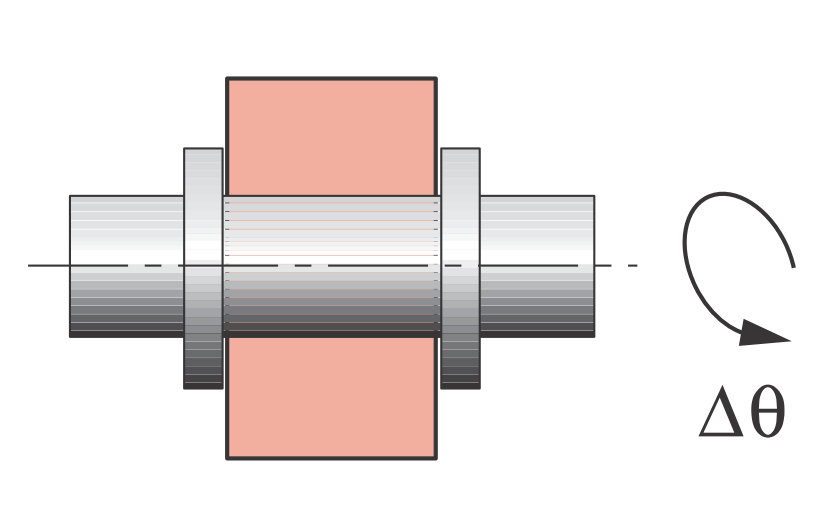
\includegraphics[height=2cm,width=1\textwidth,keepaspectratio]{R_joint.png}
            \caption{Revolute (R) joint --- 1 DoF}
            \label{fig:R_joint.png}
        \end{subfigure}
        \begin{subfigure}{0.32\textwidth}
            \centering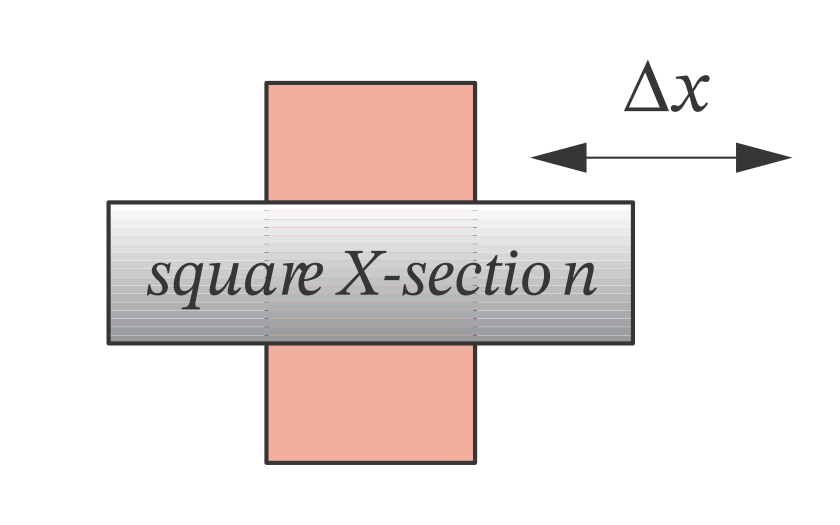
\includegraphics[height=2cm,width=1\textwidth,keepaspectratio]{P_joint.png}
            \caption{Prismatic (P) joint --- 1 DoF}
            \label{fig:P_joint.png}
        \end{subfigure}
        \begin{subfigure}{0.32\textwidth}
            \centering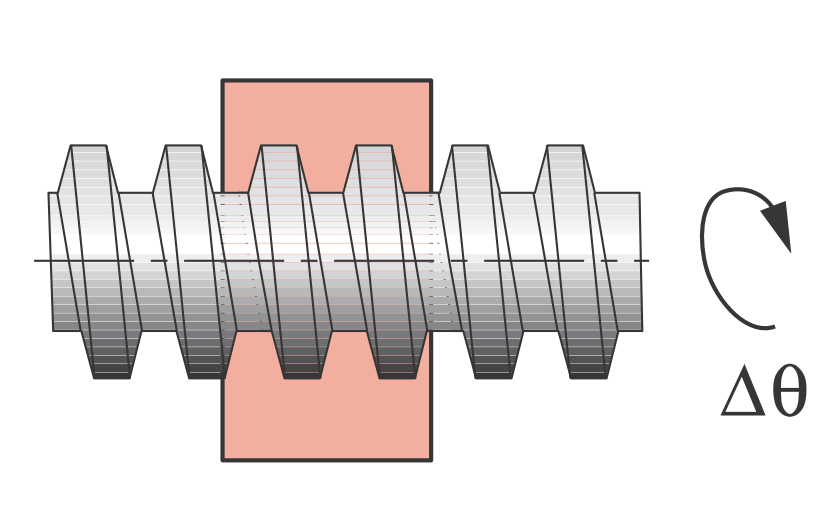
\includegraphics[height=2cm,width=1\textwidth,keepaspectratio]{H_joint.png}
            \caption{Helical (screw) (H) joint --- 1 DoF}
            \label{fig:H_joint.png}
        \end{subfigure}

        \begin{subfigure}{0.32\textwidth}
            \centering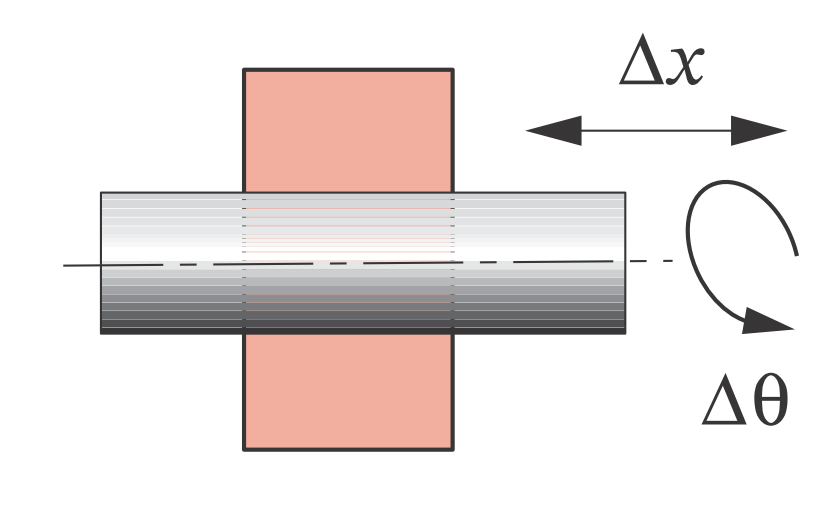
\includegraphics[height=2cm,width=1\textwidth,keepaspectratio]{C_joint.png}
            \caption{Cylindrical (C) joint --- 2 DoF}
            \label{fig:C_joint.png}
        \end{subfigure}
        \begin{subfigure}{0.32\textwidth}
            \centering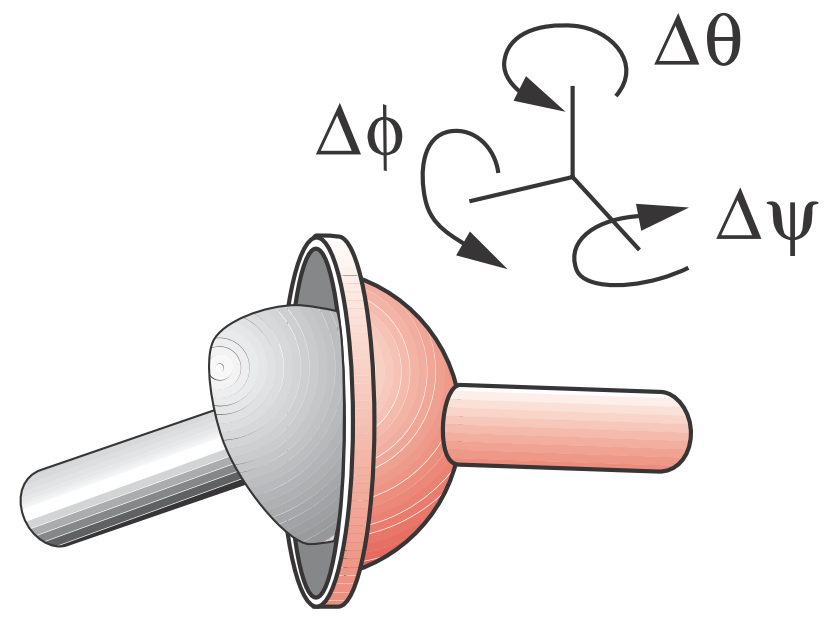
\includegraphics[height=2cm,width=1\textwidth,keepaspectratio]{S_joint.png}
            \caption{Spherical (S) joint --- 3 DoF}
            \label{fig:S_joint.png}
        \end{subfigure}
        \begin{subfigure}{0.32\textwidth}
            \centering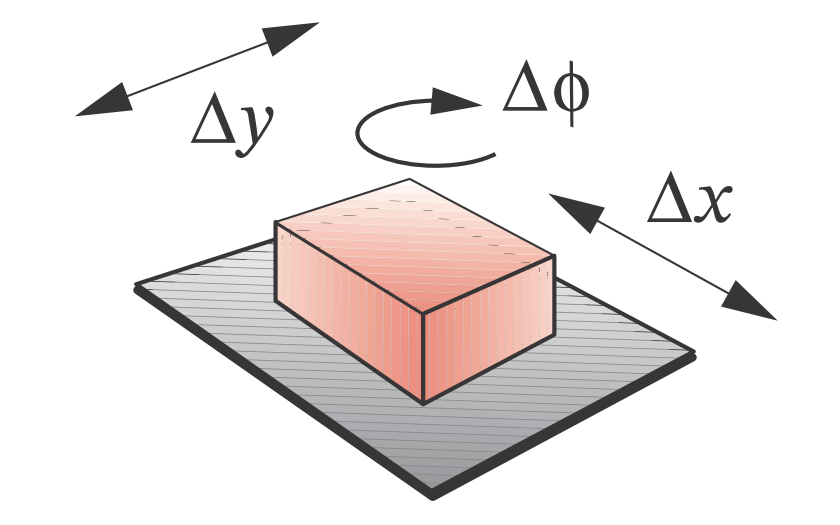
\includegraphics[height=2cm,width=1\textwidth,keepaspectratio]{F_joint.png}
            \caption{Planar (F) joint --- 3 DoF}
            \label{fig:F_joint.png}
        \end{subfigure}
    \end{figure}
\end{frame}

\begin{frame}[t]{Kinematic Pairs}
    \framesubtitle{Higher kinematic pairs (some examples)}
    \vspace{-0.3cm}
    Term \textbf{Higher pair} to describe joints with point or line contact (toothed gears)
    \vspace{-0.3cm}

    \begin{figure}[H]
        \begin{subfigure}{0.32\textwidth}
            \centering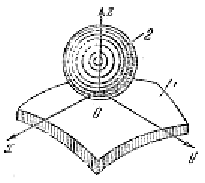
\includegraphics[height=2.5cm,width=1\textwidth,keepaspectratio]{hkp_1.png}
            \label{fig:hkp_1.png}
        \end{subfigure}
        \begin{subfigure}{0.32\textwidth}
            \centering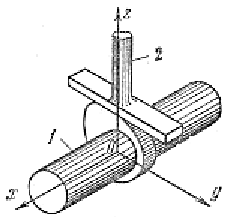
\includegraphics[height=2.5cm,width=1\textwidth,keepaspectratio]{hkp_2.png}
            \label{fig:hkp_2.png}
        \end{subfigure}
        \begin{subfigure}{0.32\textwidth}
            \centering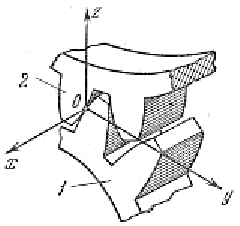
\includegraphics[height=2.5cm,width=1\textwidth,keepaspectratio]{hkp_3.png}
            \label{fig:hkp_3.png}
        \end{subfigure}

        \begin{subfigure}{0.32\textwidth}
            \centering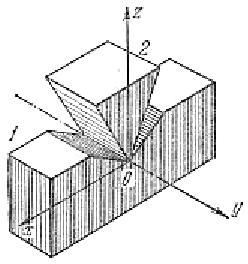
\includegraphics[height=2.5cm,width=1\textwidth,keepaspectratio]{hkp_4.png}
            \label{fig:hkp_4.png}
        \end{subfigure}
        \begin{subfigure}{0.32\textwidth}
            \centering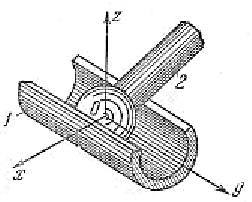
\includegraphics[height=2.5cm,width=1\textwidth,keepaspectratio]{hkp_5.png}
            \label{fig:hkp_5.png}
        \end{subfigure}
        \begin{subfigure}{0.32\textwidth}
            \centering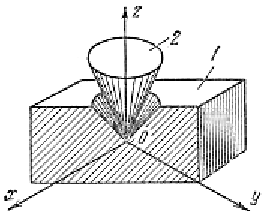
\includegraphics[height=2.5cm,width=1\textwidth,keepaspectratio]{hkp_6.png}
            \label{fig:hkp_6.png}
        \end{subfigure}
    \end{figure}
\end{frame}

\begin{frame}[t]{Kinematic Pairs}
\framesubtitle{Type of closures}
\vspace{-0.5cm}
    \begin{figure}[H]
        \begin{subfigure}[t]{0.49\textwidth}
            \centering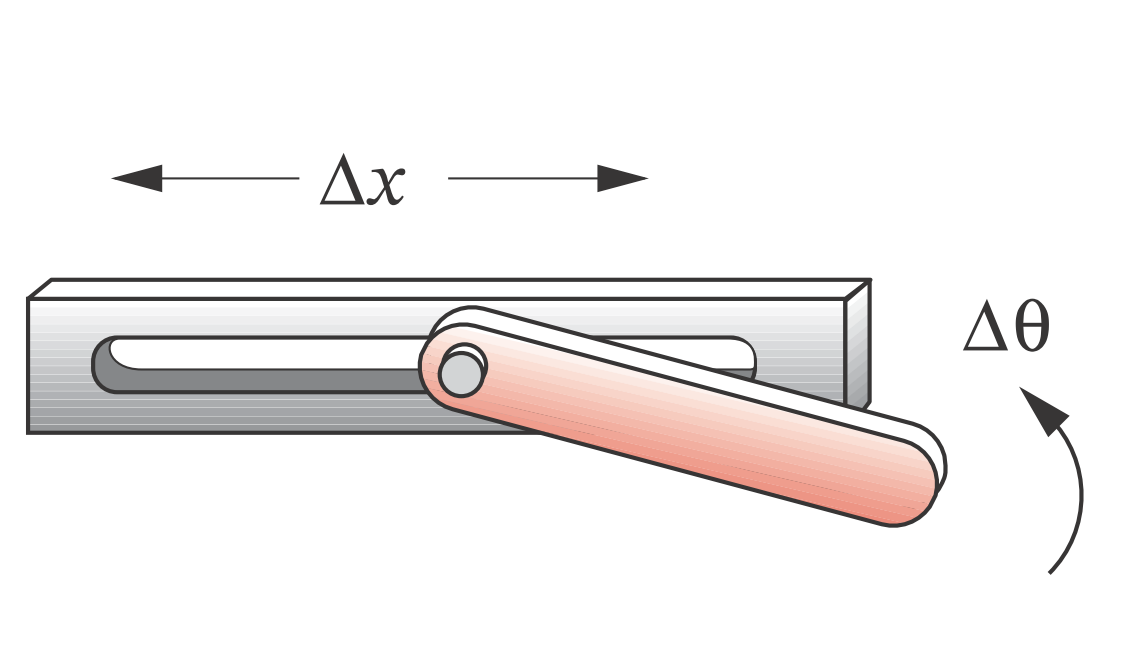
\includegraphics[height=4cm,width=1\textwidth,keepaspectratio]{RP_form_closed.png}
            \caption*{\textbf{Form-closed} joint is kept together or \textit{closed by its geometry}}
            \label{fig:RP_form_closed.png}
        \end{subfigure}
        \begin{subfigure}[t]{0.49\textwidth}
            \centering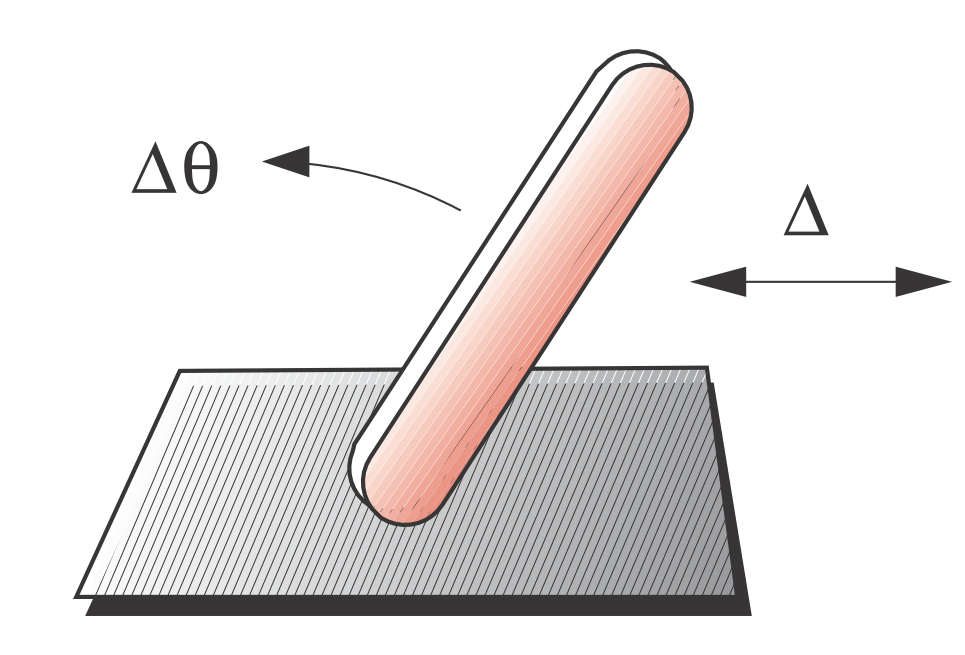
\includegraphics[height=4cm,width=1\textwidth,keepaspectratio]{RP_force_closed.png}
            \caption*{\textbf{Forced-closed} joint requires some \textit{external force to keep} it together or closed.  This force could be supplied by gravity, a spring, or any external means}
            \label{fig:RP_force_closed.png}
        \end{subfigure}
    \end{figure}
\end{frame}

\begin{frame}[t]{Kinematic Pairs}
    \framesubtitle{Joint class}
    \vspace{-0.5cm}
    \begin{table}[H]
        \centering
        \resizebox{\linewidth}{!}{%
        \begin{tabular}{c|cccc}
        \multicolumn{1}{c}{} & \begin{tabular}[c]{@{}c@{}}\textbf{No}\\\textbf{Translational }\\\textbf{Constraints}\end{tabular} & \begin{tabular}[c]{@{}c@{}}\textbf{1}\\\textbf{Translational}\\\textbf{Constraint}\end{tabular} & \begin{tabular}[c]{@{}c@{}}\textbf{2}\\\textbf{Translational}\\\textbf{Constraint}\end{tabular} & \begin{tabular}[c]{@{}c@{}}\textbf{3}\\\textbf{Translational}\\\textbf{Constraint}\end{tabular} \\ 
        \cline{2-5}
        \begin{tabular}[c]{@{}c@{}}\textbf{No}\\\textbf{Rotational Constraints}\end{tabular} & \begin{tabular}[c]{@{}c@{}}\uncover<2->{No kinematic pair,\\~free bodies}\end{tabular} & \uncover<2->{I Class} & \uncover<2->{II Class} & \uncover<2->{III Class} \\
        \begin{tabular}[c]{@{}c@{}}\textbf{1}\\\textbf{Rotational Constraint}\end{tabular} & \uncover<2->{\underline{Impossible}} & \uncover<2->{II~Class} & \uncover<2->{III~Class} & \uncover<2->{IV~Class} \\
        \begin{tabular}[c]{@{}c@{}}\textbf{2}\\\textbf{Rotational Constraint}\end{tabular} & \uncover<2->{\underline{Impossible}} & \uncover<2->{III~Class} & \uncover<2->{IV~Class} & \uncover<2->{V~Class} \\
        \begin{tabular}[c]{@{}c@{}}\textbf{3}\\\textbf{Rotational Constraint}\end{tabular} & \uncover<2->{\underline{Impossible}} & \uncover<2->{\underline{Impossible}} & \uncover<2->{V~Class} & \uncover<2->{Fixed joint}
        \end{tabular}
        }
    \end{table}
\end{frame}

\begin{frame}[t]{Skeleton Diagrams}
\framesubtitle{Definition}
\vspace{-0.3cm}
A \textbf{skeleton diagram} is a simplified drawing of a mechanism or machine that shows only
the dimensions that affect its kinematics.

The connecting rod and piston both
have many geometric features, mostly associated with issues of strength and the size of
the bearing at each joint. These features are kinematically unimportant.
\vspace{-0.5cm}

\begin{figure}[H]
    \centering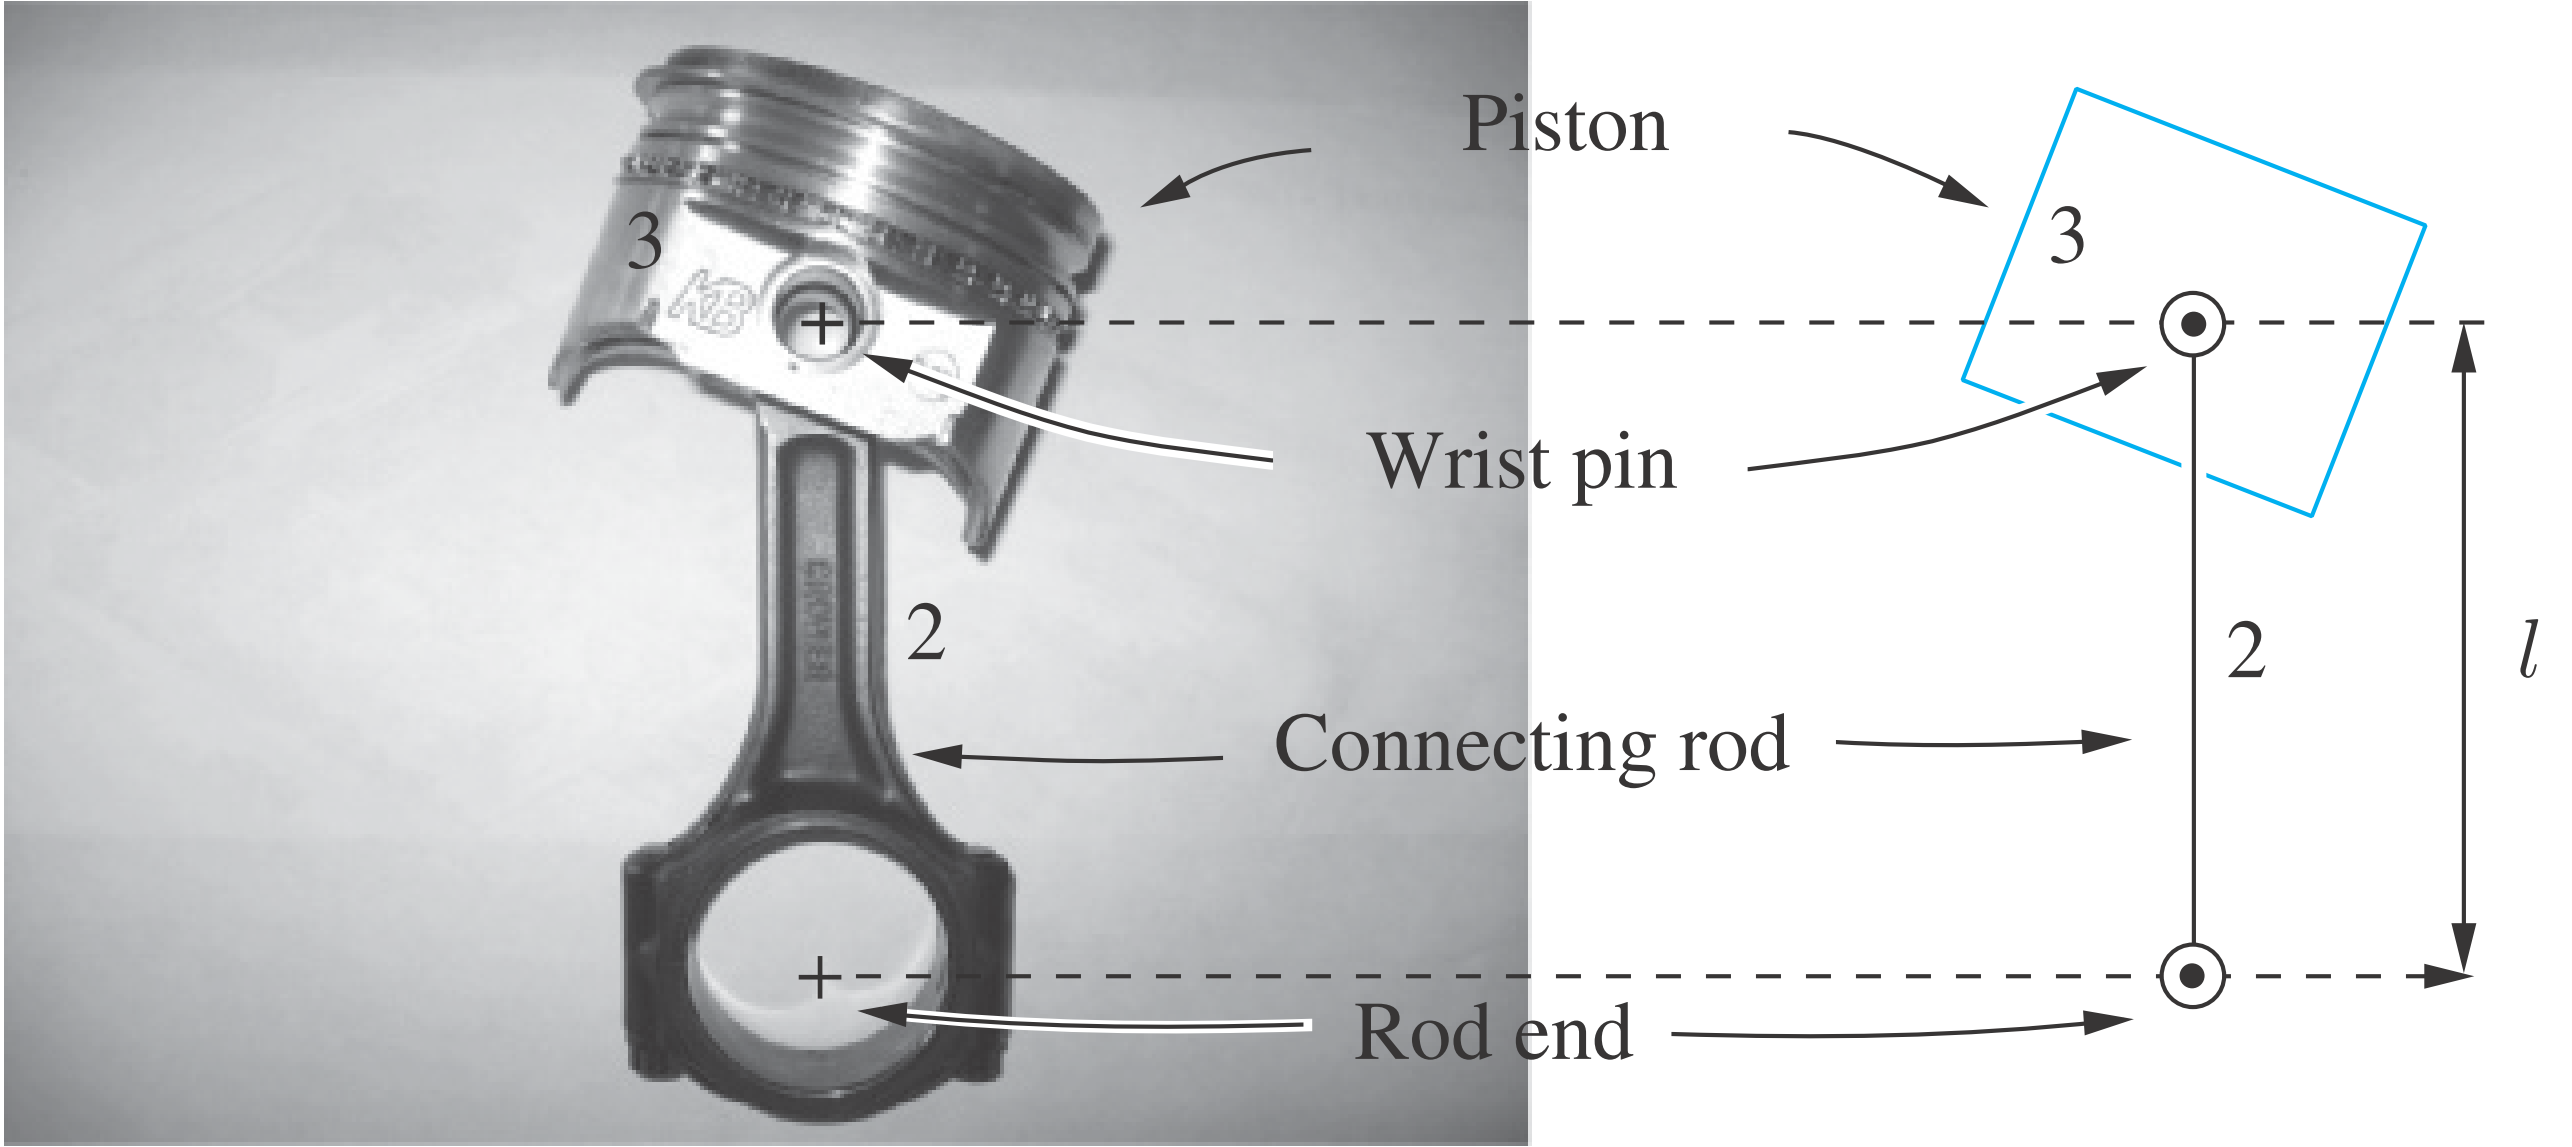
\includegraphics[height=3.5cm,width=1\textwidth,keepaspectratio]{skeleton_diagram.png}
    % \caption{caption_name}
    \label{fig:skeleton_diagram.png}
\end{figure}
\end{frame}

\begin{frame}[t]{Skeleton Diagrams}
    \framesubtitle{Russian notation (1)}
    \vspace{-0.5cm}
    \begin{figure}[H]
        \begin{subfigure}{0.32\textwidth}
            \centering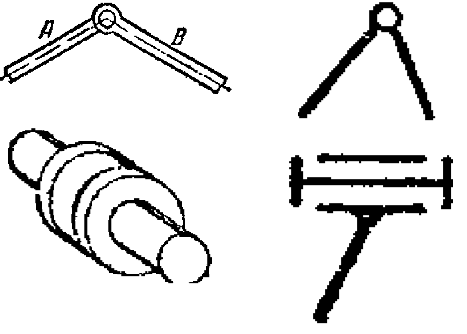
\includegraphics[height=2.2cm,width=1\textwidth,keepaspectratio]{R_sd.png}
            \caption*{R joint}
        \end{subfigure}
        \begin{subfigure}{0.32\textwidth}
            \centering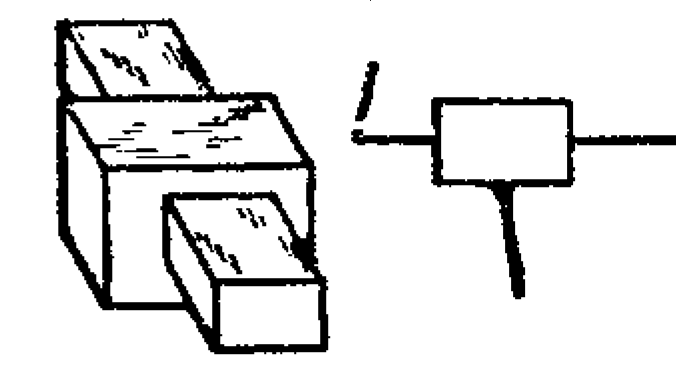
\includegraphics[height=2.2cm,width=1\textwidth,keepaspectratio]{P_sd.png}
            \caption*{P joint}
        \end{subfigure}
        \begin{subfigure}{0.32\textwidth}
            \centering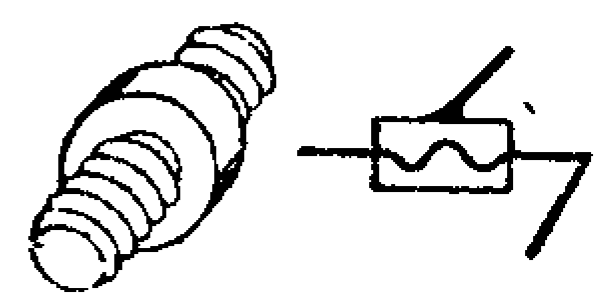
\includegraphics[height=2.2cm,width=1\textwidth,keepaspectratio]{H_sd.png}
            \caption*{H joint}
        \end{subfigure}
    
        \begin{subfigure}{0.32\textwidth}
            \centering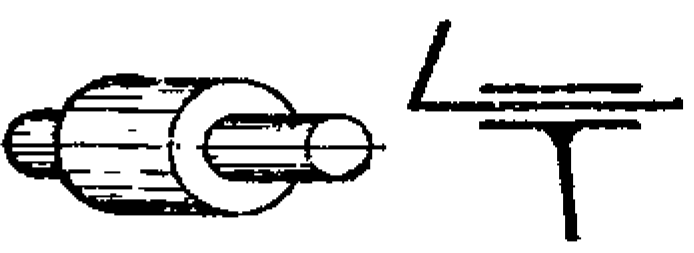
\includegraphics[height=2.2cm,width=1\textwidth,keepaspectratio]{C_sd.png}
            \caption*{C joint}
        \end{subfigure}
        \begin{subfigure}{0.32\textwidth}
            \centering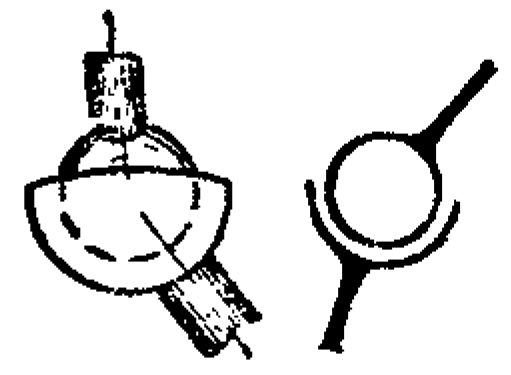
\includegraphics[height=2.2cm,width=1\textwidth,keepaspectratio]{S_sd.png}
            \caption*{S joint}
        \end{subfigure}
        \begin{subfigure}{0.32\textwidth}
            \centering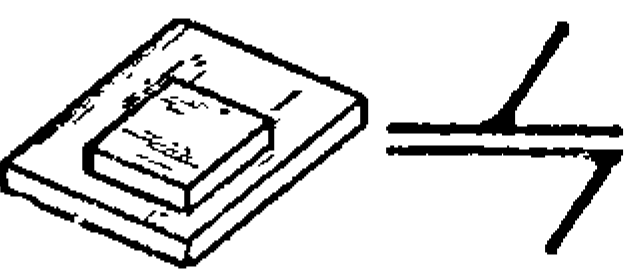
\includegraphics[height=2.2cm,width=1\textwidth,keepaspectratio]{F_sd.png}
            \caption*{F joint}
        \end{subfigure}
    \end{figure}
    \end{frame}

\begin{frame}[t]{Skeleton Diagrams}
\framesubtitle{Russian notation (2)}
\vspace{-0.5cm}
\begin{figure}[H]
    \begin{subfigure}{0.32\textwidth}
        \centering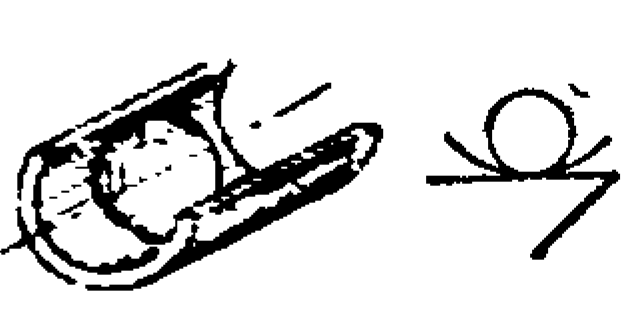
\includegraphics[height=2.2cm,width=1\textwidth,keepaspectratio]{B_C_sd.png}
        \caption*{Ball-Cylinder joint}
    \end{subfigure}
    \begin{subfigure}{0.32\textwidth}
        \centering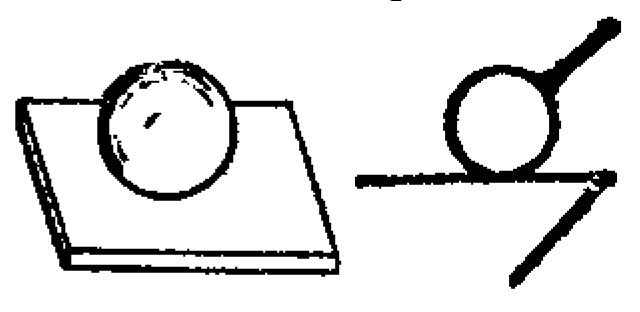
\includegraphics[height=2.2cm,width=1\textwidth,keepaspectratio]{B_F_sd.png}
        \caption*{Ball-Plane joint}
    \end{subfigure}
    \begin{subfigure}{0.32\textwidth}
        \centering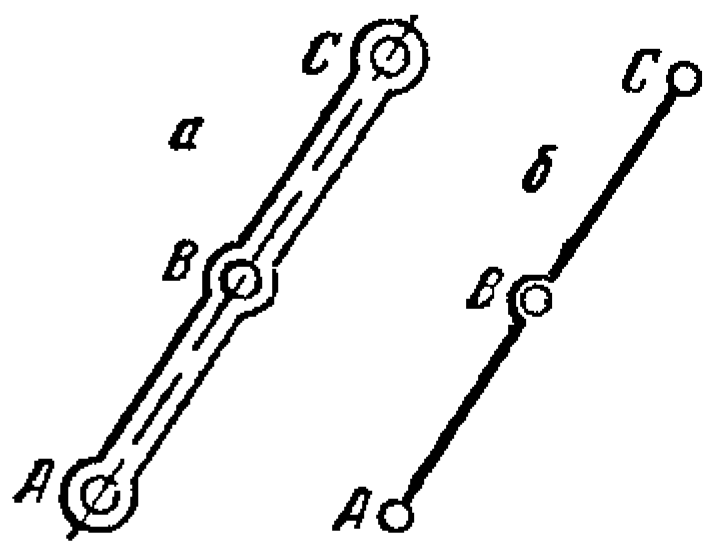
\includegraphics[height=2.2cm,width=1\textwidth,keepaspectratio]{3l_sd.png}
        \caption*{3 node link}
    \end{subfigure}


    \begin{subfigure}{0.32\textwidth}
        \centering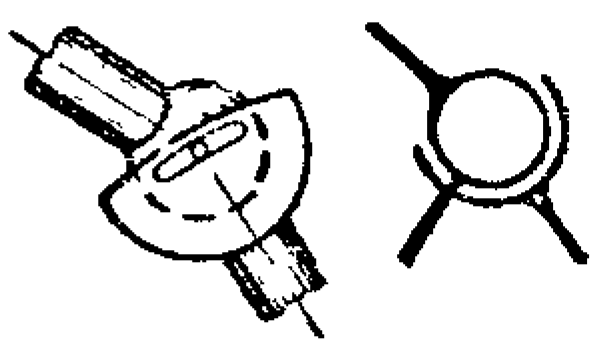
\includegraphics[height=2.2cm,width=1\textwidth,keepaspectratio]{Smin_sd.png}
        \caption*{S with extra link joint}
    \end{subfigure}
    \begin{subfigure}{0.32\textwidth}
        \centering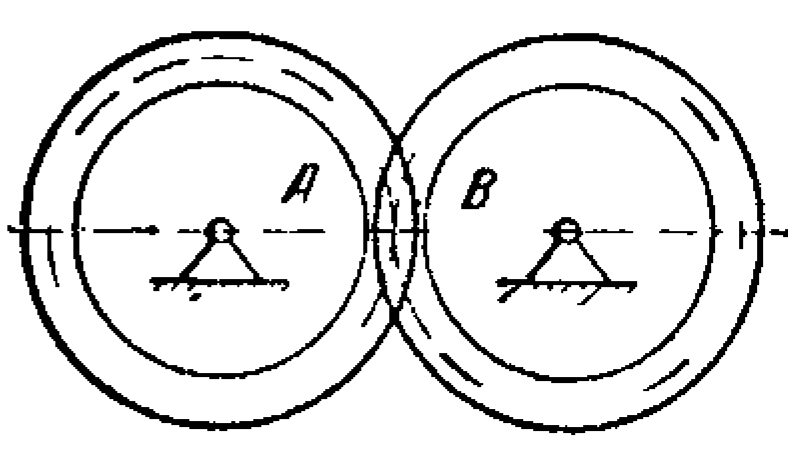
\includegraphics[height=2.2cm,width=1\textwidth,keepaspectratio]{Tooth_sd.png}
        \caption*{Gear transmission}
    \end{subfigure}
    \begin{subfigure}{0.32\textwidth}
        \centering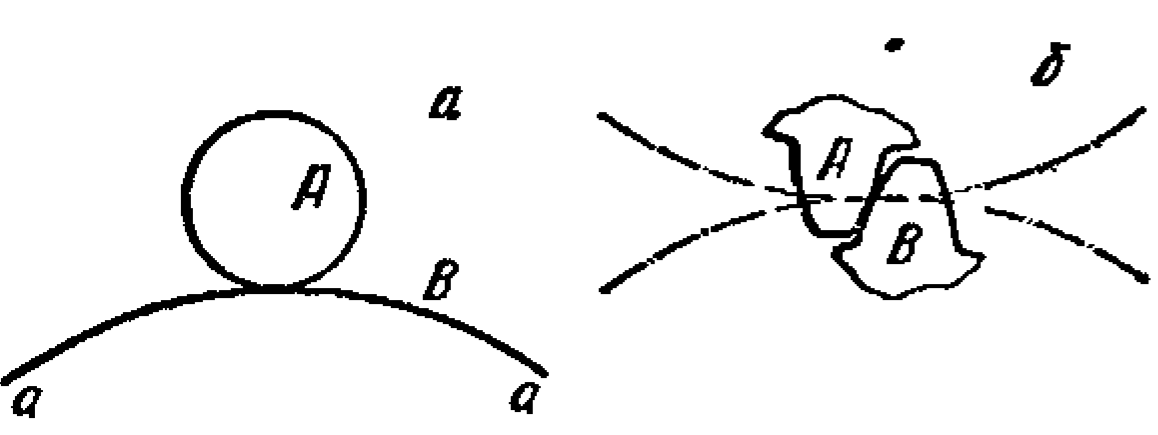
\includegraphics[height=2.2cm,width=1\textwidth,keepaspectratio]{Higher_sd.png}
        \caption*{R joint with base}
    \end{subfigure}
\end{figure}
\end{frame}

\begin{frame}[t]{Skeleton Diagrams}
\framesubtitle{Examples (Russian)}
\vspace{-0.5cm}
    \begin{figure}[H]
        \begin{subfigure}[c]{0.49\textwidth}
            \centering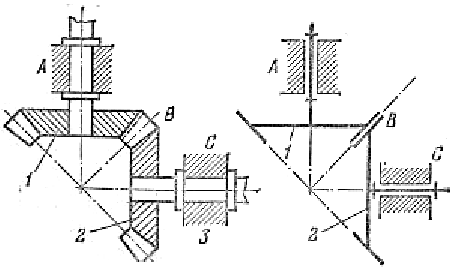
\includegraphics[height=6cm,width=1\textwidth,keepaspectratio]{rus1_mech.png}
            \label{fig:rus1_mech.png}
        \end{subfigure}
        \begin{subfigure}[c]{0.49\textwidth}
            \centering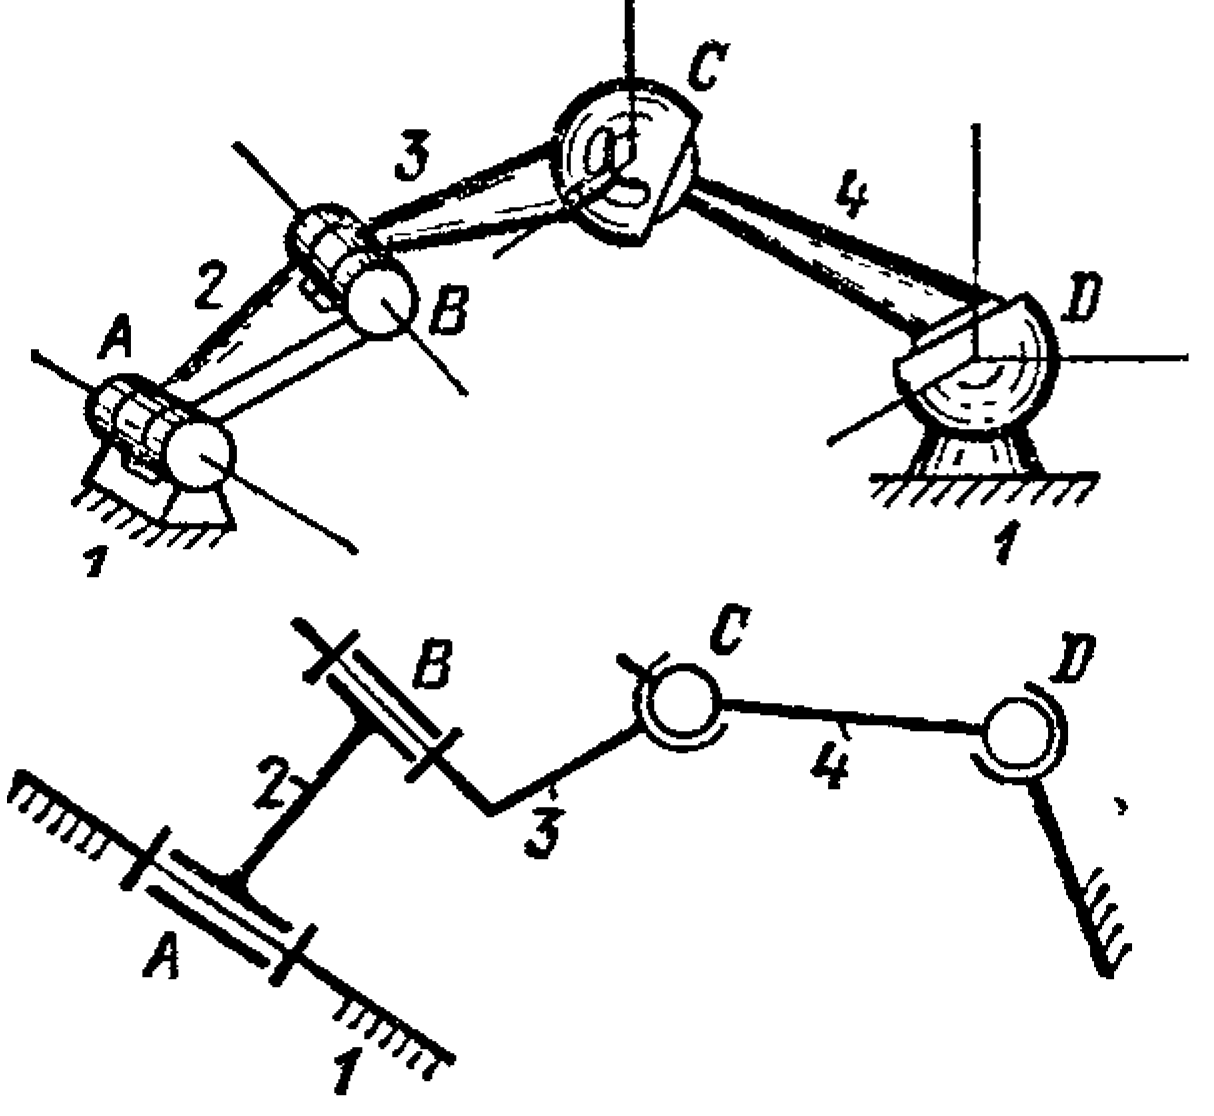
\includegraphics[height=6cm,width=1\textwidth,keepaspectratio]{rus2_mech.png}
            \label{fig:rus2_mech.png}
        \end{subfigure}
    \end{figure}
\end{frame}

\begin{frame}[t]{Skeleton Diagrams}
    \framesubtitle{Examples (Foreign)}
    \vspace{-0.5cm}
    \begin{figure}[H]
        \begin{subfigure}{0.49\textwidth}
            \centering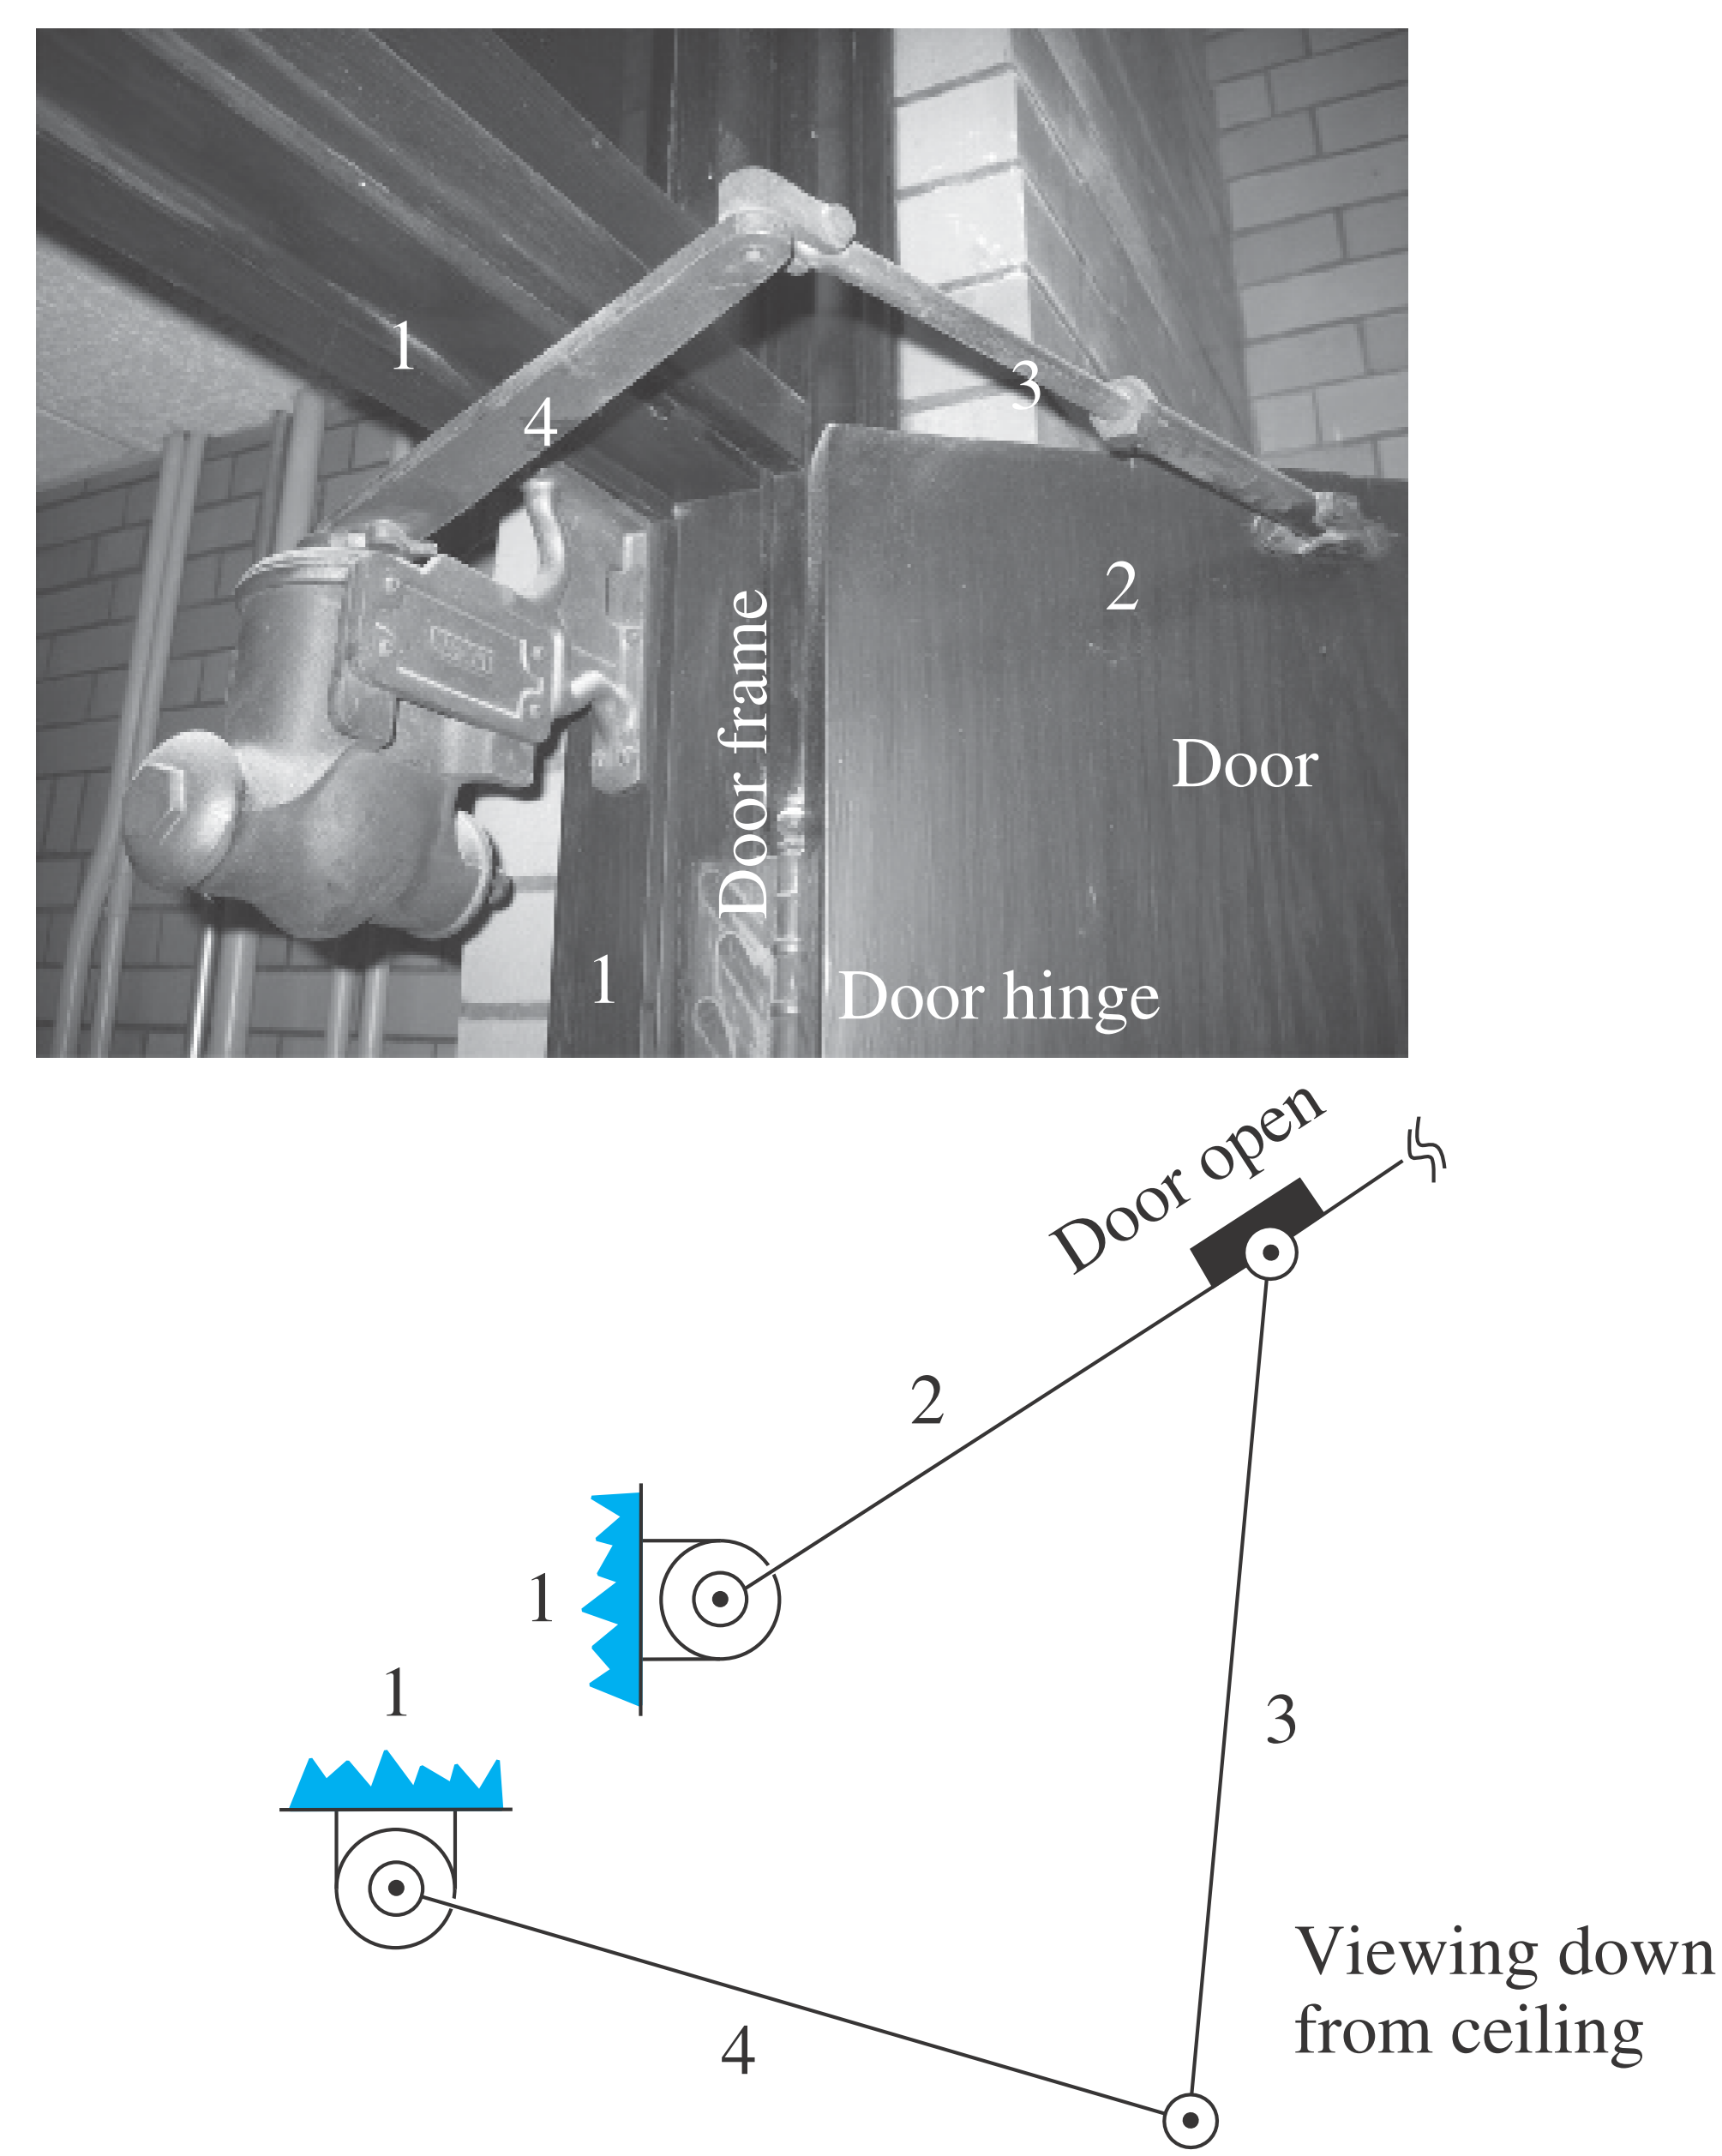
\includegraphics[height=6cm,width=1\textwidth,keepaspectratio]{en1_mech.png}
            \label{fig:en1_mech.png}
        \end{subfigure}
        \begin{subfigure}{0.49\textwidth}
            \centering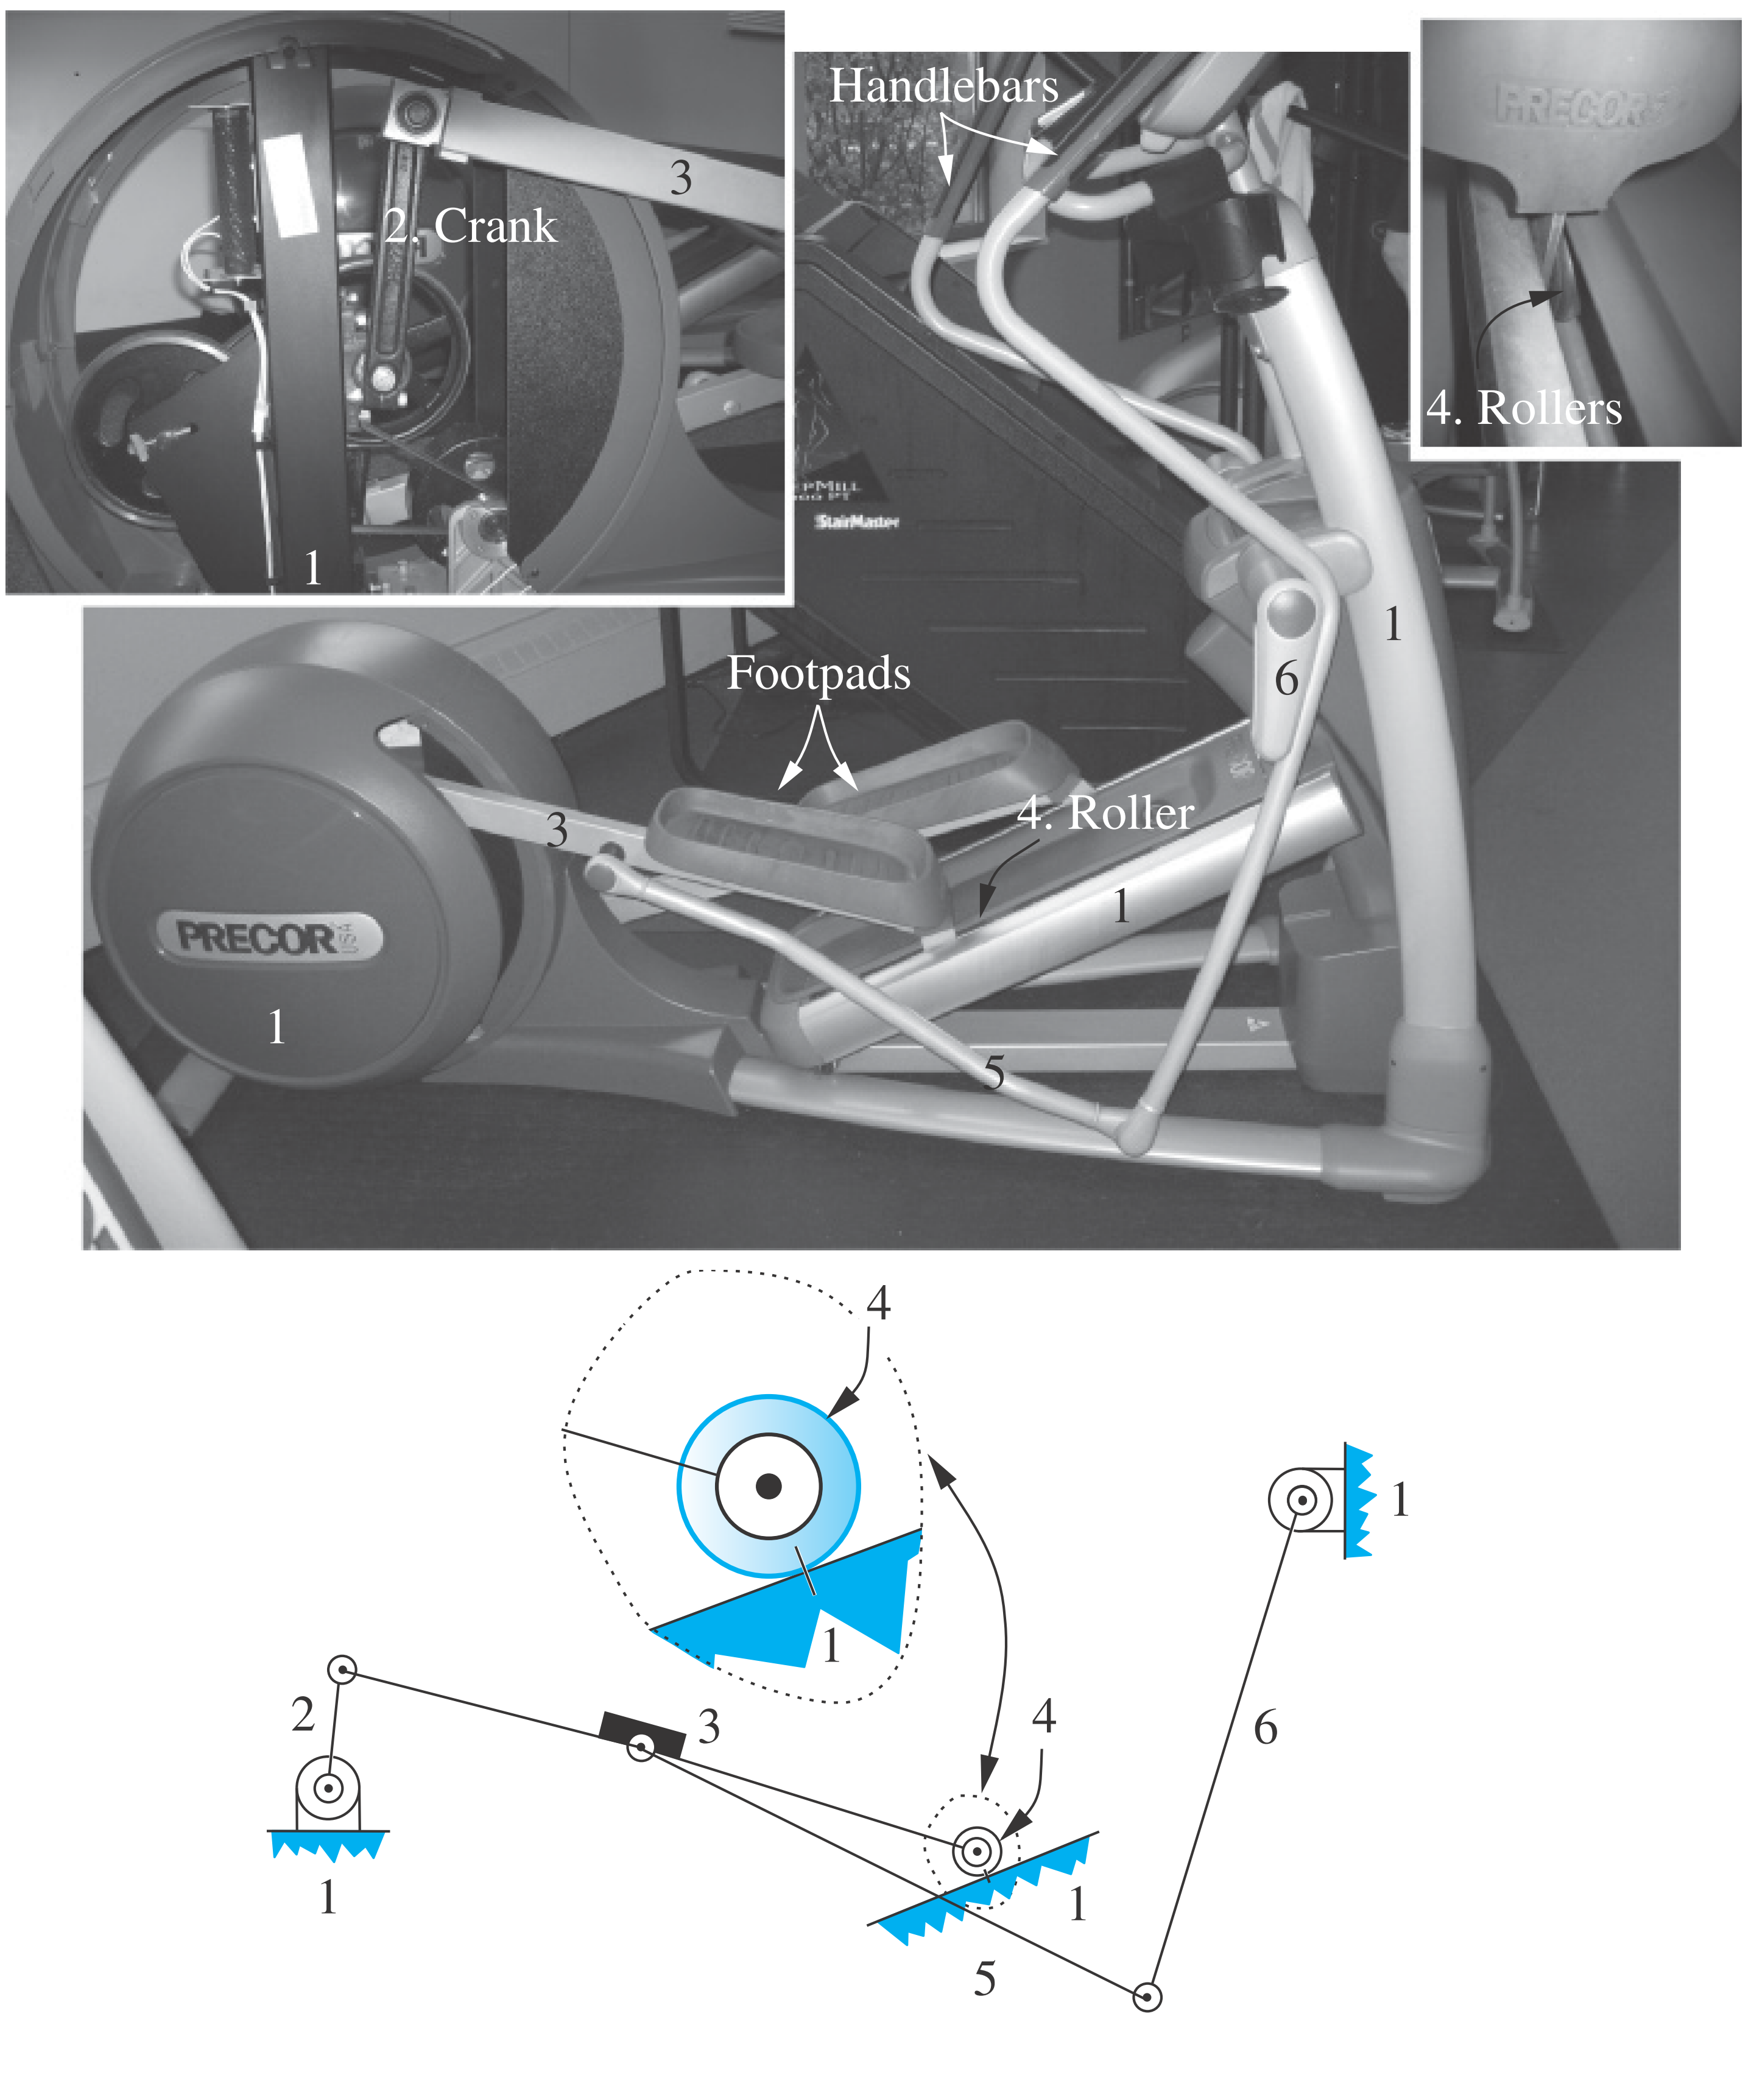
\includegraphics[height=6cm,width=1\textwidth,keepaspectratio]{en2_mech.png}
            \label{fig:en2_mech.png}
        \end{subfigure}
    \end{figure}       
    \end{frame}

\begin{frame}[t]{Kinematic Chains}
\framesubtitle{Definitions}
\textbf{Kinematic chain} is an assemblage of links and joints interconnected in a way to provide a controlled output motion in response to a supplied input motion.

A \textit{\textbf{closed} Kinematic chain} will have no open attachment 
points or nodes and may have one or more degrees of freedom.

An \textit{\textbf{open} Kinematic chain} of more than one link will always have more than one degree of freedom, thus requiring as many actuators (motors) as it has DoF.
\end{frame}

\begin{frame}[t]{Kinematic Chains}
    \framesubtitle{Examples}
    \vspace{-0.5cm}
        \begin{figure}[H]
            \begin{subfigure}{0.49\textwidth}
                \centering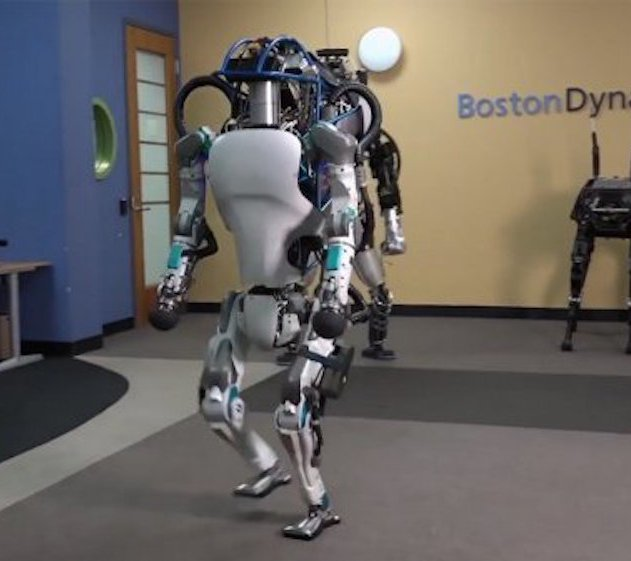
\includegraphics[height=3cm,width=1\textwidth,keepaspectratio]{kc_1.png}
                % \caption{capture1}
                \label{fig:kc_1.png}
            \end{subfigure}
            \begin{subfigure}{0.49\textwidth}
                \centering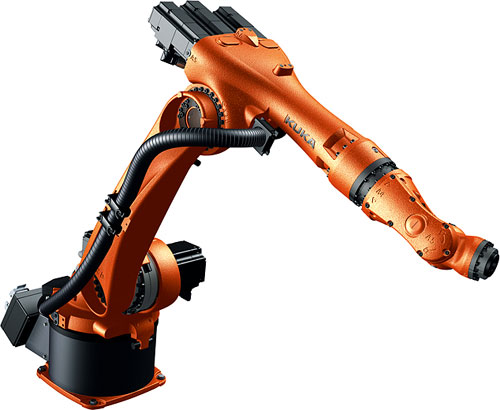
\includegraphics[height=3cm,width=1\textwidth,keepaspectratio]{kc_2.png}
                % \caption{capture2}
                \label{fig:kc_2.png}
            \end{subfigure}
 
            \begin{subfigure}{0.49\textwidth}
                \centering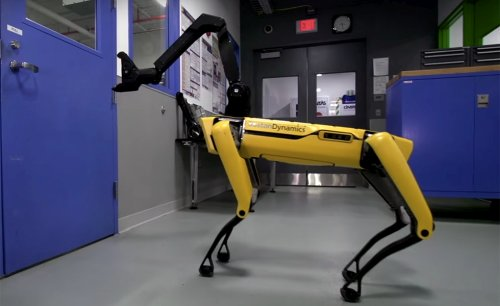
\includegraphics[height=3cm,width=1\textwidth,keepaspectratio]{kc_3.png}
                % \caption{capture1}
                \label{fig:kc_3.png}
            \end{subfigure}
            \begin{subfigure}{0.49\textwidth}
                \centering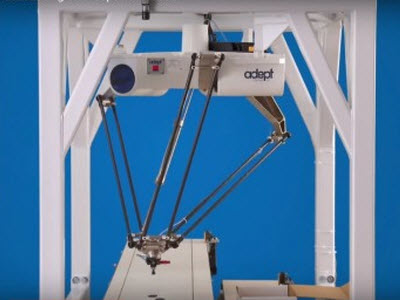
\includegraphics[height=3cm,width=1\textwidth,keepaspectratio]{kc_4.png}
                % \caption{capture2}
                \label{fig:kc_4.png}
            \end{subfigure}
        \end{figure}
    \end{frame}

\begin{frame}[t]{Degrees of Freedom}
    \framesubtitle{Definitions}
        DoF --- the number of independent coordinates required to define its position.

        \begin{align*}
            \text{DoF}=m(N-1-J) + \sum_{i=1}^{J}f_i,
        \end{align*}
        where $N$ --- \# of bodies, including ground;
        
        $J$ --- \# of joints;
        
        $m$ --- eq. to 3 if planar mech, 6 -- spatial;
        
        $f_i$ --- DoF of the joint.
    \end{frame}


\begin{frame}[t]{Degrees of Freedom}
    \framesubtitle{Video}
    \vspace{-0.6cm}
    \begin{figure}[H]
        \href{https://youtu.be/zI64DyaRUvQ}{
            \centering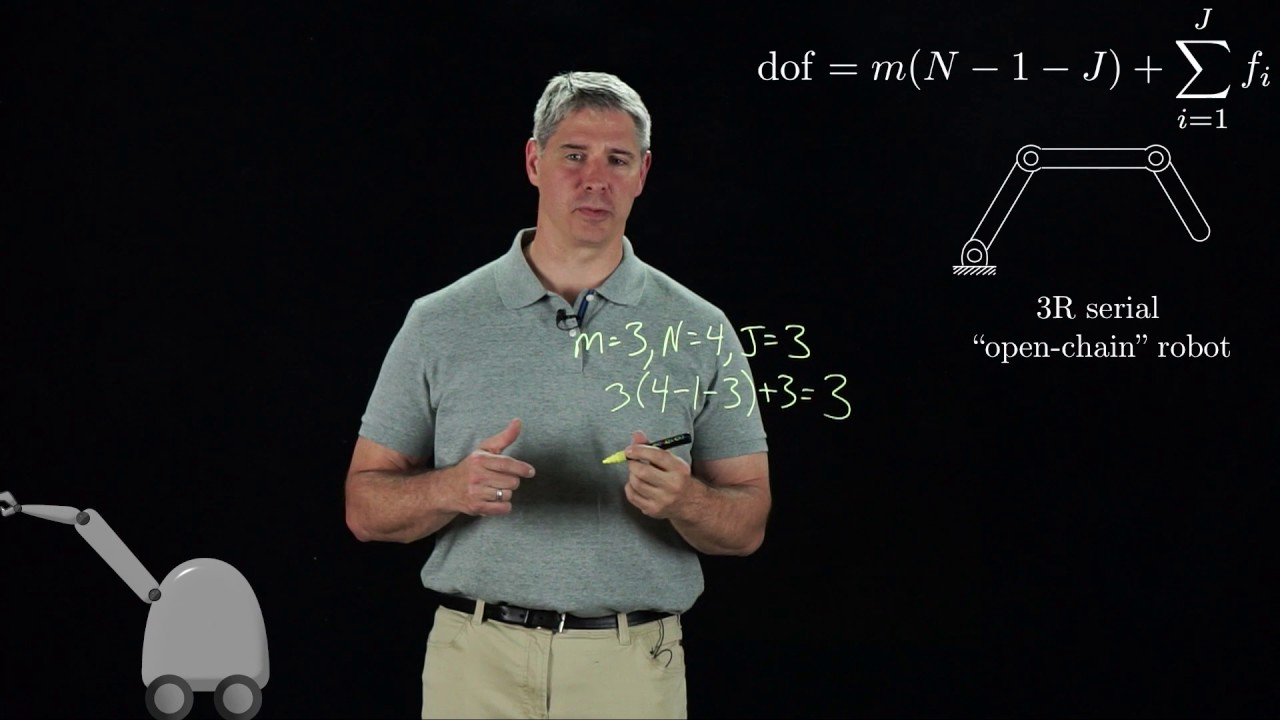
\includegraphics[height=6cm,width=1\textwidth,keepaspectratio]{dof_video.jpg}}
        % \caption{Click on a picture for a video}
        \label{fig:dof_video.jpg}
    \end{figure}
\end{frame}

\begin{frame}[t]{Degrees of Freedom}
    \framesubtitle{Example}
    \vspace{-0.5cm}
    \begin{figure}[H]
            \centering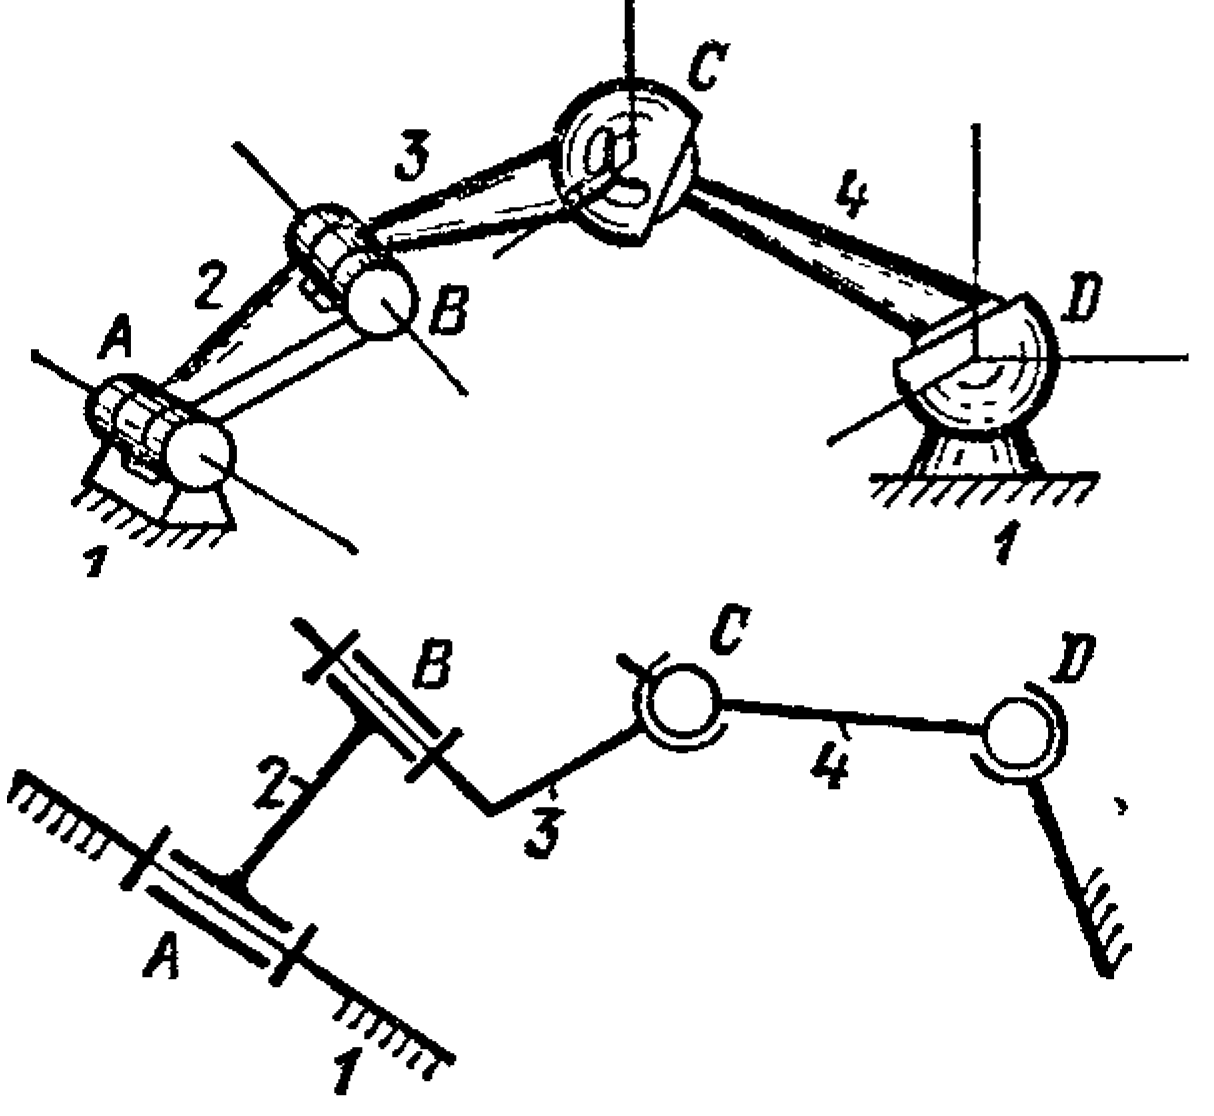
\includegraphics[height=5cm,width=1\textwidth,keepaspectratio]{rus2_mech.png}
            \caption*{$\text{DoF}=6(4-1-4) + (1+1+2+3) = 1$}
    \end{figure}
    \end{frame}

\begin{frame}[t]{Degrees of Freedom}
    \framesubtitle{Practical Task}
    \vspace{-0.7cm}
    \begin{figure}[H]
        \centering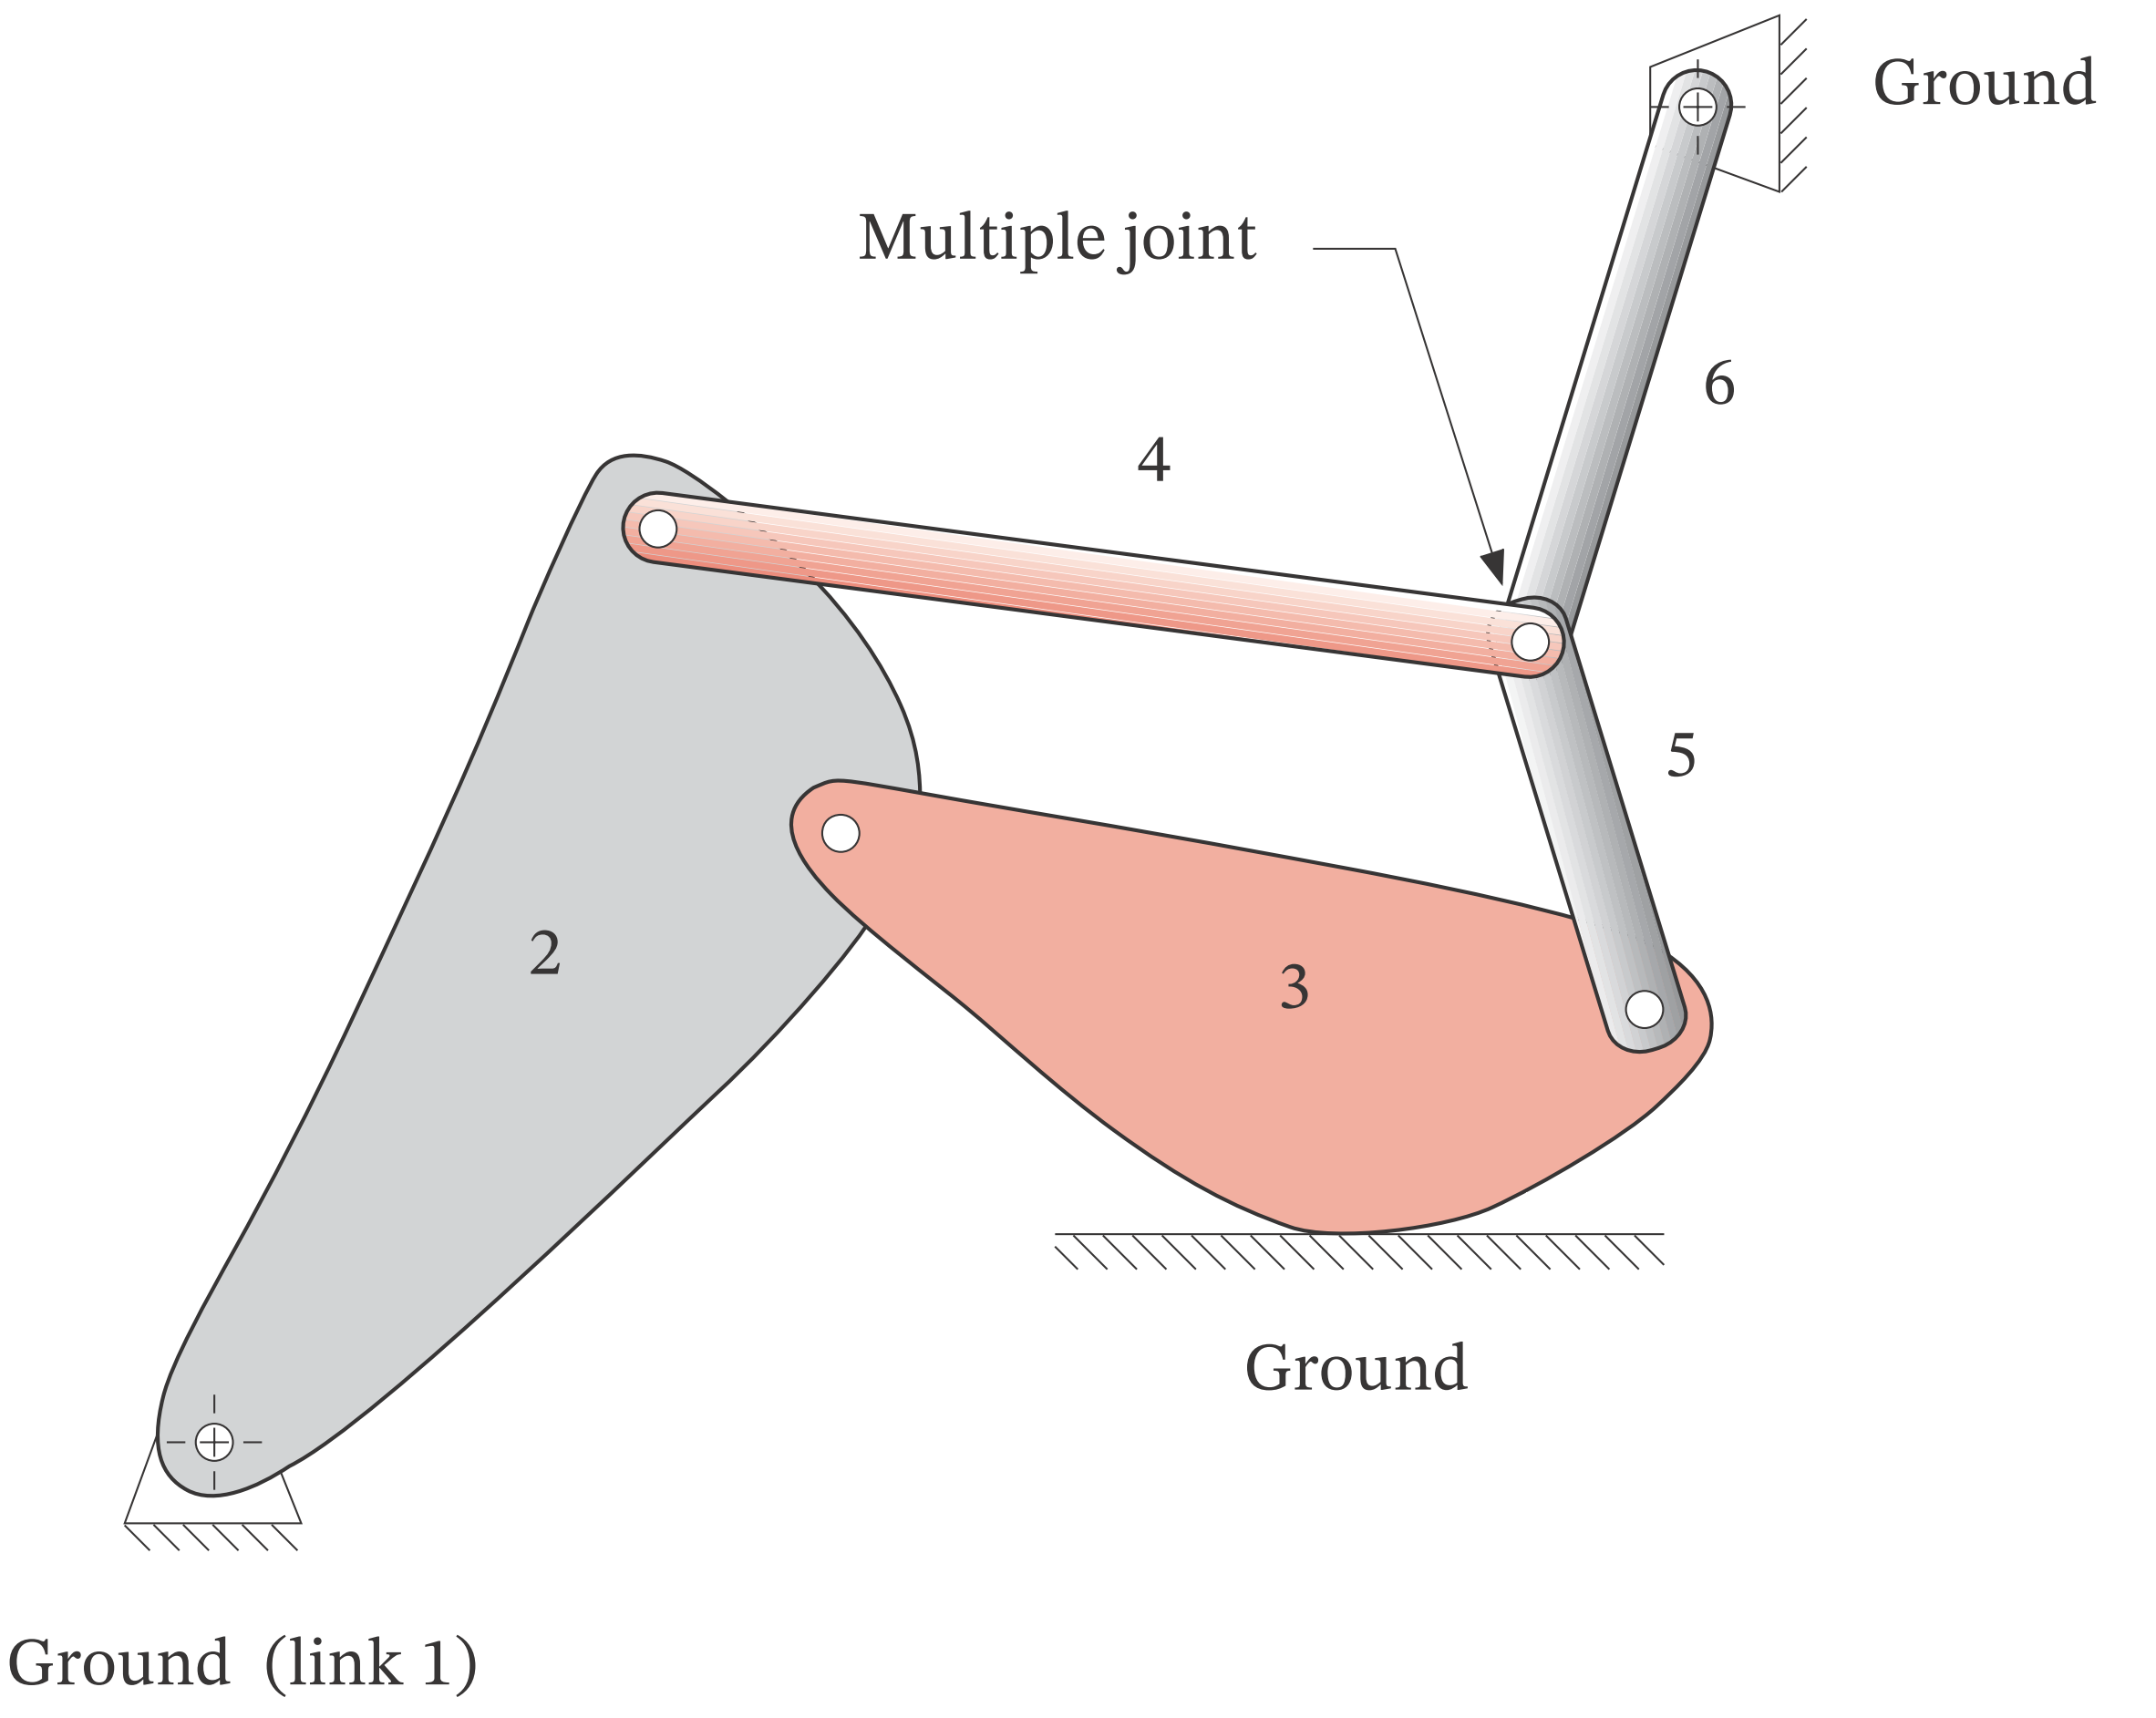
\includegraphics[height=5.5cm,width=1\textwidth,keepaspectratio]{stud_task.png}
        \caption*{\uncover<2->{$\text{DoF}=3(6-1-8) + (2+7*1) = 0$}}
        \label{fig:stud_task.png}
    \end{figure}        
    \end{frame}

    
\begin{frame}[t]{Degrees of Freedom}
    \framesubtitle{Not working with classical theory}
    \vspace{-0.5cm}
        \begin{figure}[H]
            \centering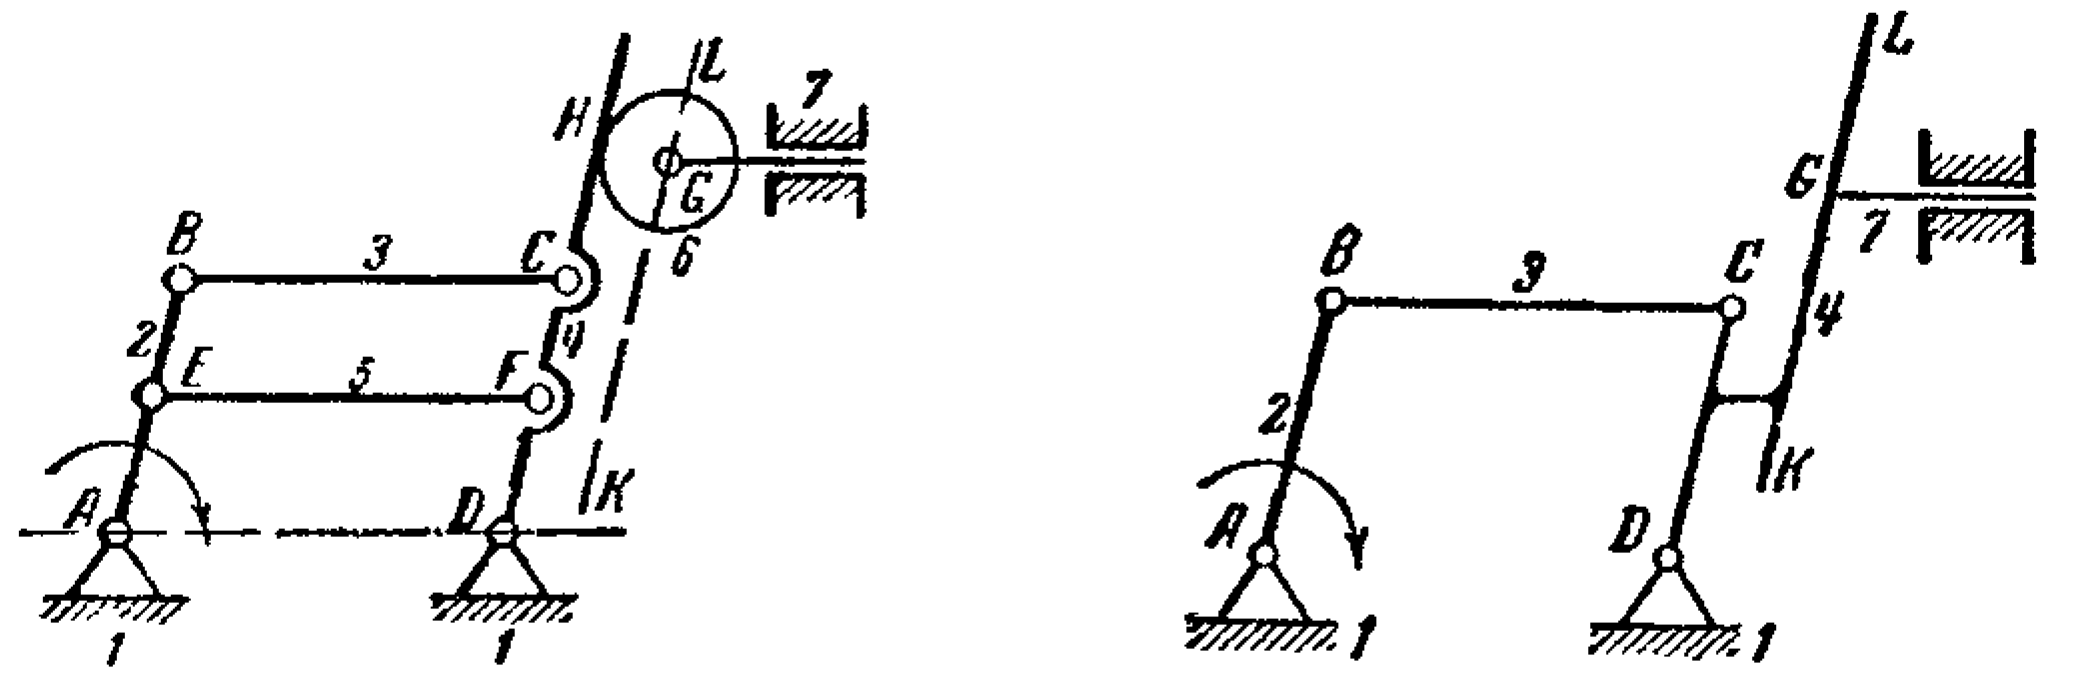
\includegraphics[height=5cm,width=1\textwidth,keepaspectratio]{extra_links_mech.png}
            % \caption{caption_name}
            \label{fig:extra_links_mech.png}
        \end{figure}
    \end{frame}

\begin{frame}[t]{Degrees of Freedom}
    \framesubtitle{Replacement of the higher joints with the lower joints}
    \vspace{-0.5cm}
        \begin{figure}[H]
            \centering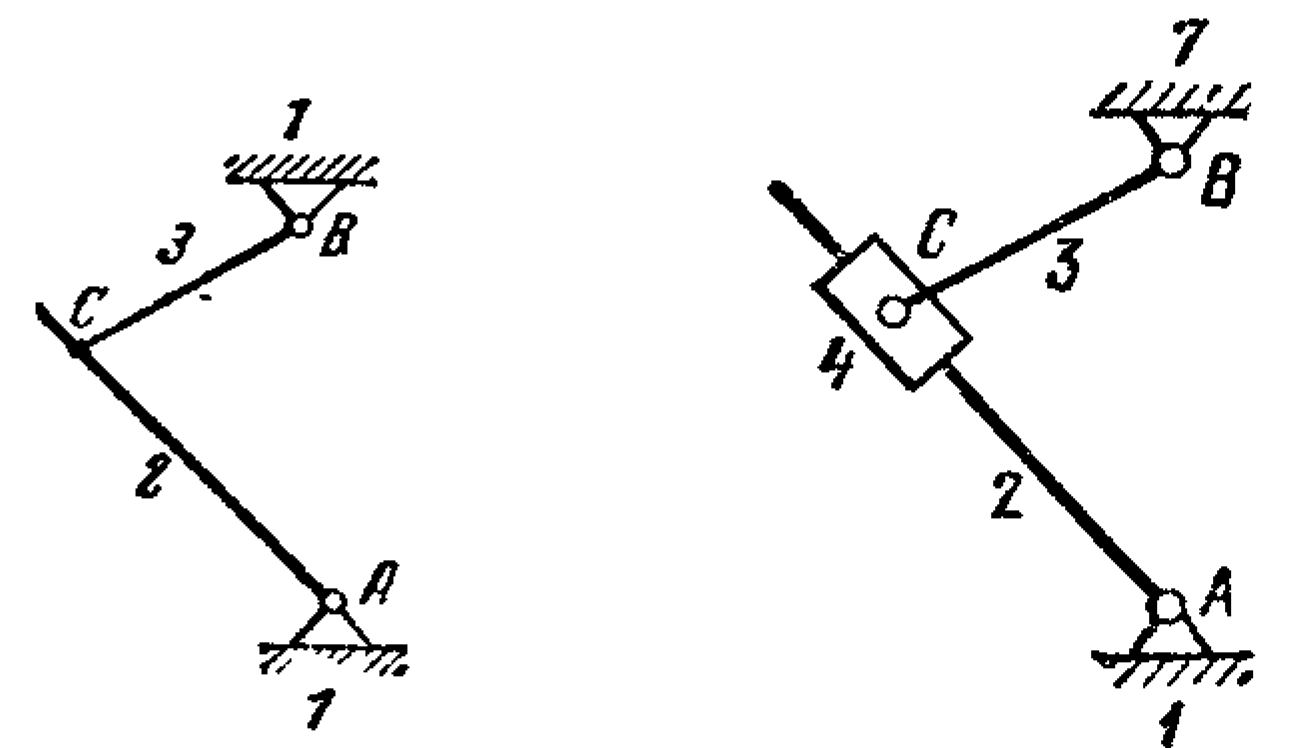
\includegraphics[height=5cm,width=1\textwidth,keepaspectratio]{from_h_to_l_mech.png}
            \caption*{From Point-Line higher joint (IV Class) to P and R lower joints (both V Class)}
            \label{from_h_to_l_mech.png}
        \end{figure}
    \end{frame}

\begin{frame}[t]{Reference material}
    % \Large
    \begin{itemize}
        \item \textit{"Mechanisms and Machines: Kinematics, Dynamics, and Synthesis" Michael M. Stanisic, pdf pages 21--56 } \textbf{1.1 --- 1.6}
        \item \textit{"Theory of Machines and Mechanisms" John J. Uicker, pdf pages 33--59 } \textbf{1.4 --- 1.7}
        \item \textit{"Design of machinery" Robert L. Norton, pdf pages 57--79 } \textbf{2.0 --- 2.11}
        \item \textit{"Механика. Теория механизмов и машин" Конищева О. В., pdf pages 7--23 } \\ Структурный анализ и классификация плоских механизмов
        \item \textit{"Теория механизмов и машин" Артоболевский И. И. 1988, pdf pages 21--63 } \\ Структурный анализ и классификация механизмов
              % \item \href{https://onlinemschool.com/math/library/vector/cos/}{Direction cosines (OnlineMSchool)}
    \end{itemize}
\end{frame}

\fbckg{fibeamer/figs/last_page.png}
\frame[plain]{}

\end{document}